% This program can be redistributed and/or modified under the terms
% of the GNU Public License, version 3.
%
% Seth Brown, Ph.D.
% sethbrown@drbunsen.org
%
% Compiled with XeLaTeX
% Dependencies:
%   Fontin Sans font (http://www.exljbris.com/fontinsans.html)
%
%\documentclass{beamer}
\documentclass[unknownkeysallowed]{beamer}

\usepackage{graphicx} % graphics
\usepackage{epsfig} % eps graphics
\usepackage{hyperref} % urls
\usepackage{booktabs, caption} % table styling

% suppress navigation bar
\beamertemplatenavigationsymbolsempty


\mode<presentation>
{
  \usetheme{bunsen}
  \setbeamercovered{transparent}
  \setbeamertemplate{items}[circle]
}

% set fonts
\usepackage{fontspec}
\setsansfont{Ubuntu}
\setbeamerfont{frametitle}{size=\LARGE,series=\bfseries}

% color definitions
\usepackage{color, soul}
\definecolor{uipoppy}{RGB}{225, 64, 5}
\definecolor{uipaleblue}{RGB}{96,123,139}
\definecolor{uiblack}{RGB}{0, 0, 0}
\definecolor{uigrey}{RGB}{192,192,192}

% caption styling
\DeclareCaptionFont{uiblack}{\color{uiblack}}
\DeclareCaptionFont{uipoppy}{\color{uipoppy}}
\captionsetup{labelfont={uipoppy},textfont=uiblack}
\setbeamercolor{section in toc}{fg=uipoppy}
\setulcolor{uipoppy}

% see the macros.tex file for definitions
% This program can be redistributed and/or modified under the terms
% of the GNU Public License, version 3.

% adds reference to bottom right of corner of a slide
\usepackage[absolute,overlay]{textpos} % text references in slide corners
\newcommand\textref[1]{%
  \begin{textblock*}{\paperwidth}(0pt,0.99\textheight)
  \raggedleft \tiny{\emph{#1}}\hspace{.5em}
  \end{textblock*}}

  %font size
  \newcommand\Fontvi{\fontsize{6}{7.2}\selectfont}
  \newcommand\Fontix{\fontsize{9}{11}\selectfont}

% for drawing circles around numbers
% ex. \circled{1} Add some text here.
\usepackage{tikz}
\newcommand*\circled[1]{\tikz[baseline=(char.base)]{
            \node[shape=circle,draw,inner sep=2pt] (char) {#1};}}


\setbeamercovered{invisible}
% title slide definition
\title{Security of Near Field Communication:\break Does My Phone Need A Tinfoil Hat?}
\author{Thomas Harren}
\institute[UMM] % (optional, but mostly needed)
{
 % \inst{1}%
  University of Minnesota, Morris
}
\date[]{April 30, 2015}

%--------------------------------------------------------------------
%                    Introduction & Outline
%--------------------------------------------------------------------

\begin{document}

\begin{frame}
  \titlepage
\end{frame}

% Set the background for the rest of the slides.
% Insert infoline
\setbeamertemplate{background}
 {
\includegraphics[width=\paperwidth,height=\paperheight]{slide_bg}}
\setbeamertemplate{footline}[bunsentheme]

\begin{frame}
\frametitle{Have you used NFC?}
  		\begin{block}{}
  		  \begin{center}
    		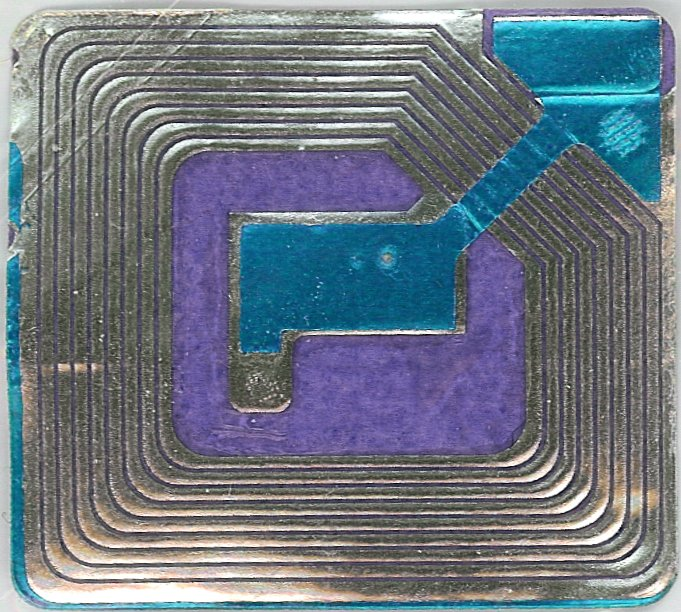
\includegraphics[width=\linewidth,height=0.3\textheight,keepaspectratio]{figures/wikimediatag.jpg}
    		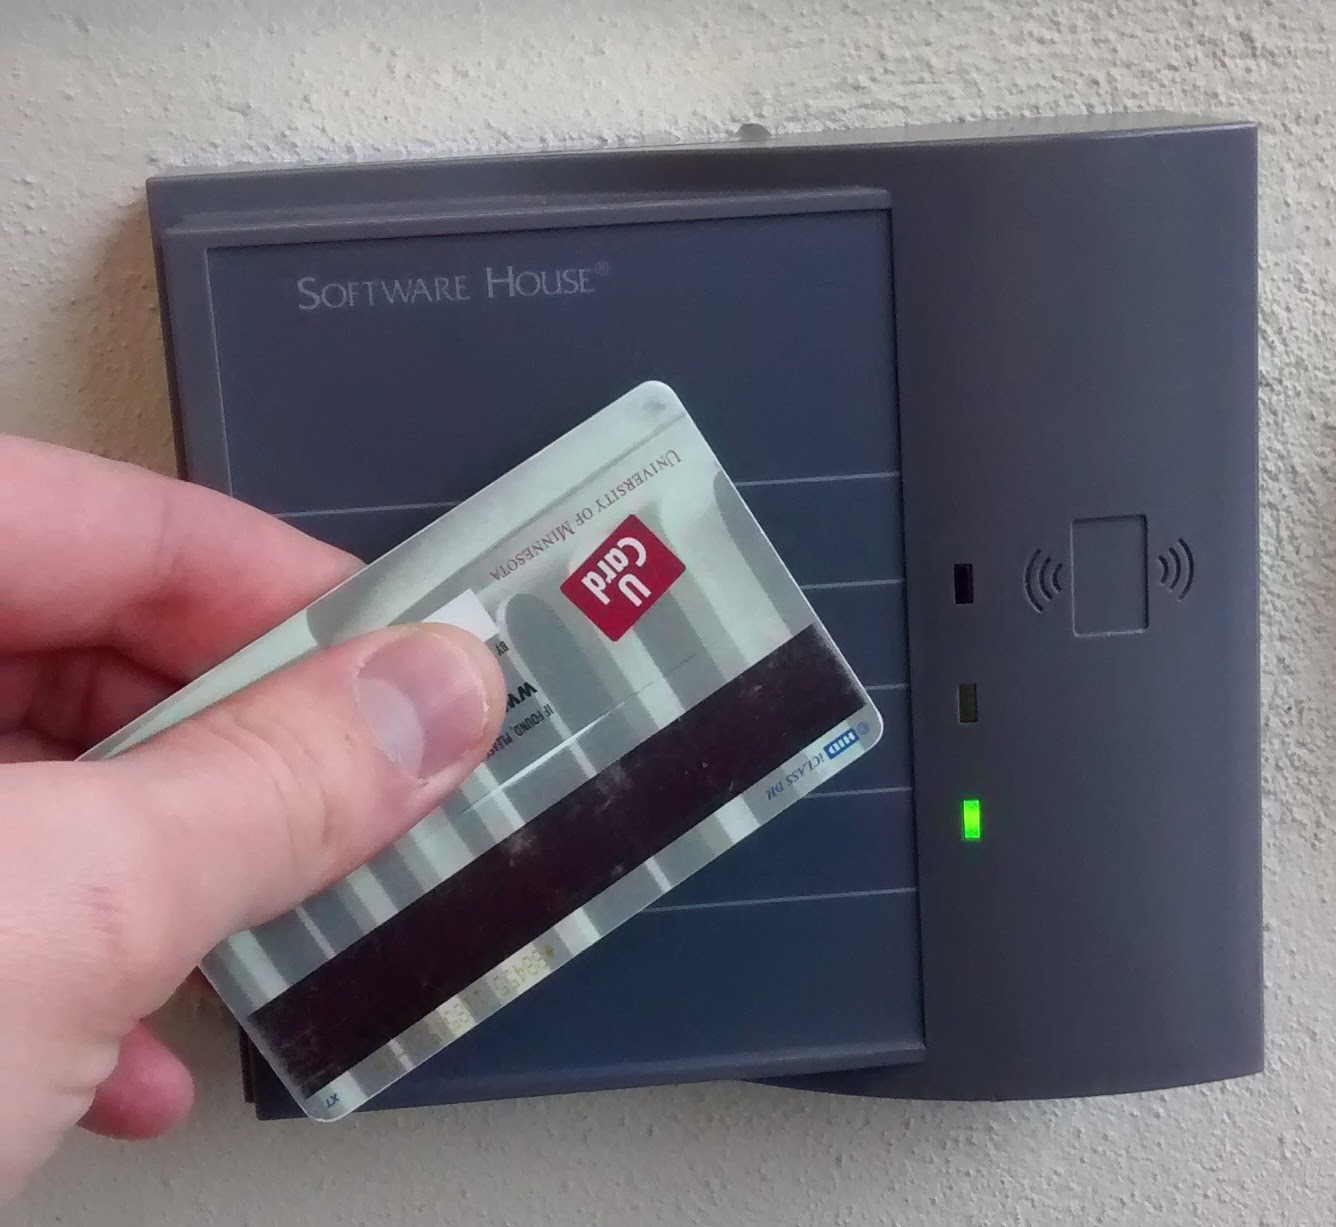
\includegraphics[width=\linewidth,height=0.3\textheight,keepaspectratio]{figures/gayHall.jpg}
        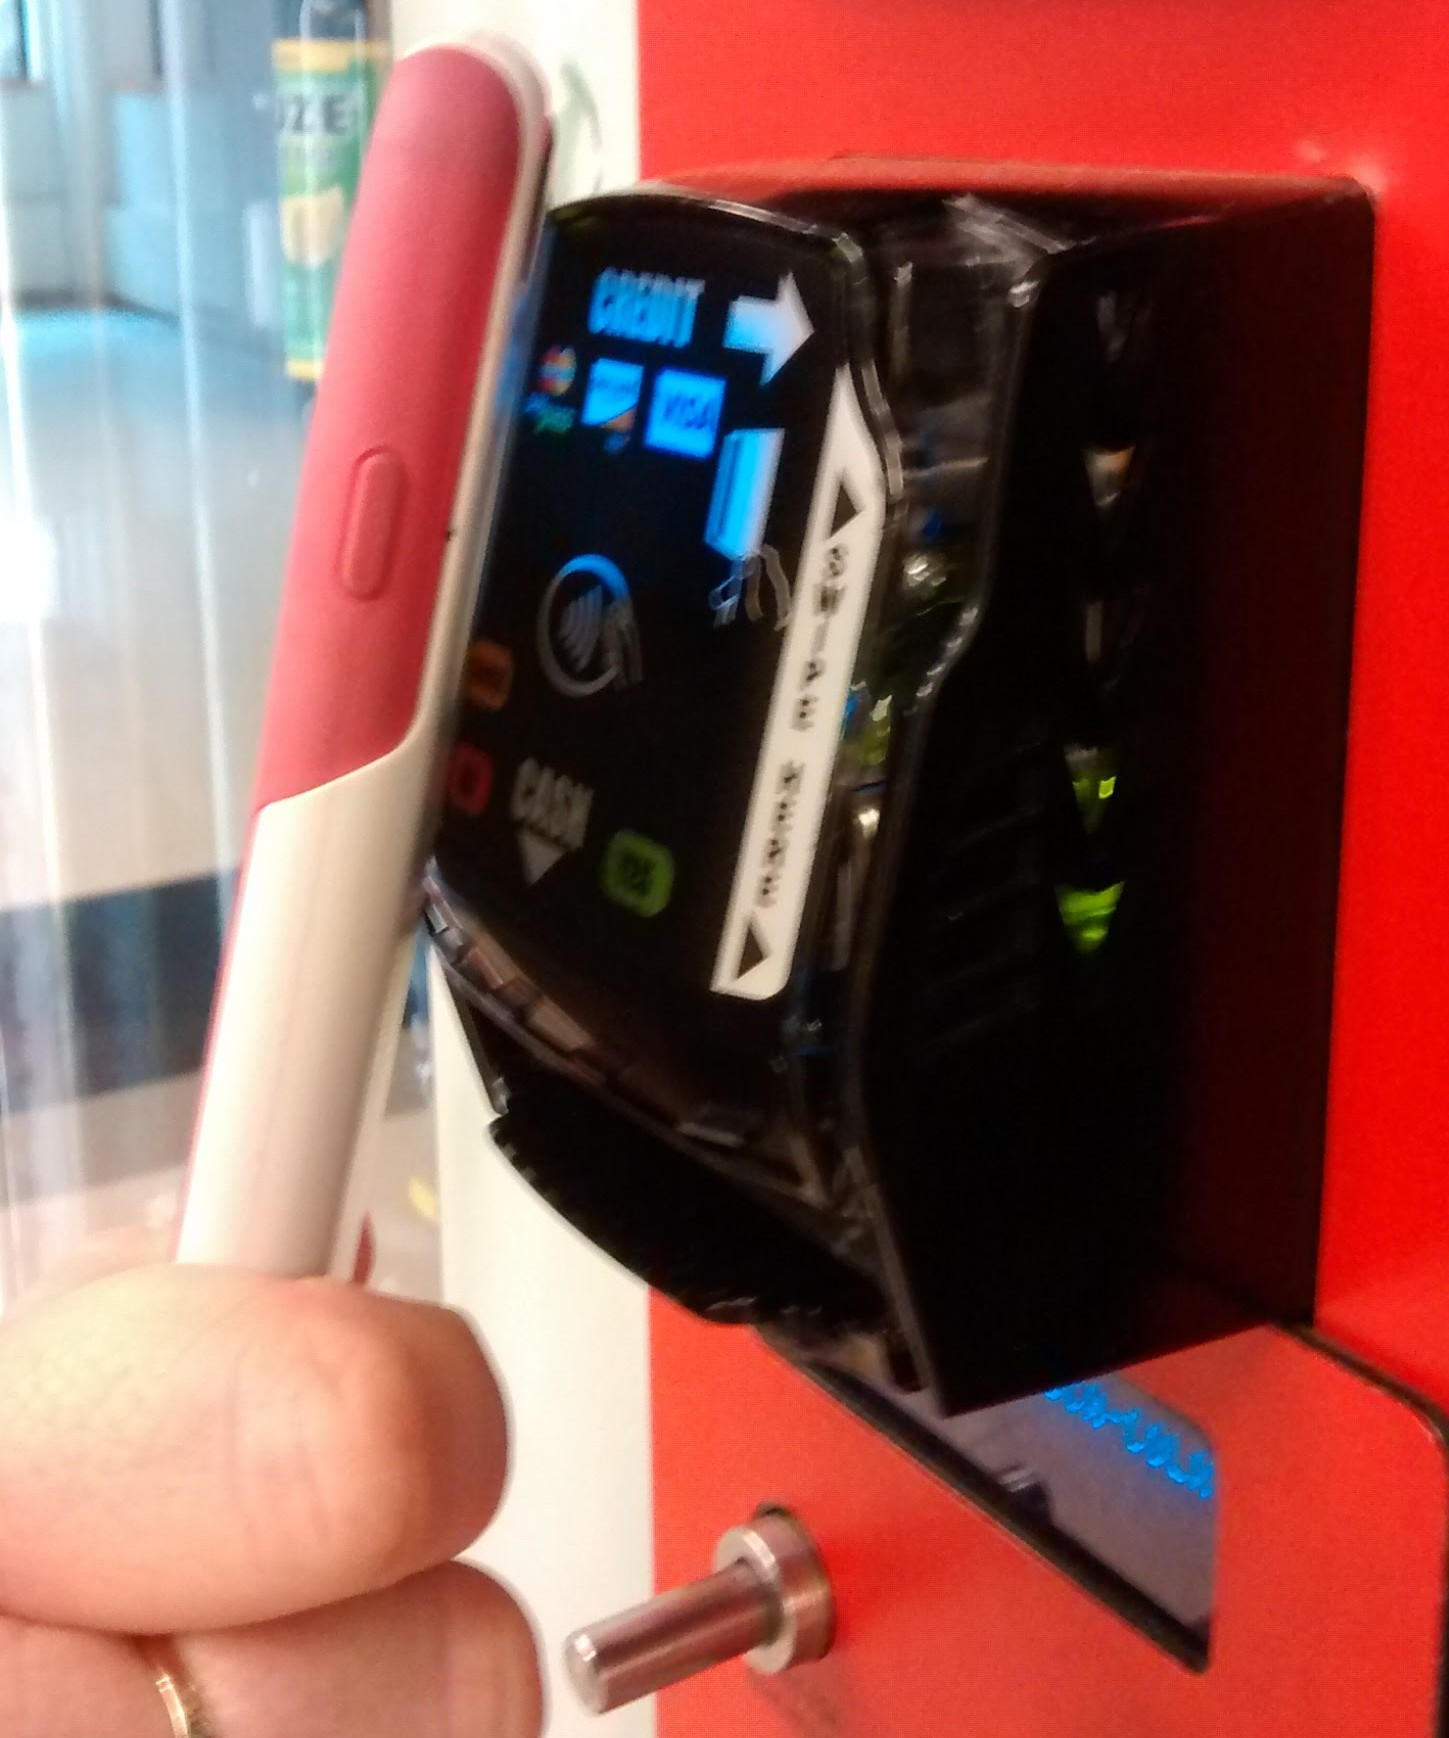
\includegraphics[width=\linewidth,height=0.3\textheight,keepaspectratio]{figures/ApplePay.jpg}
        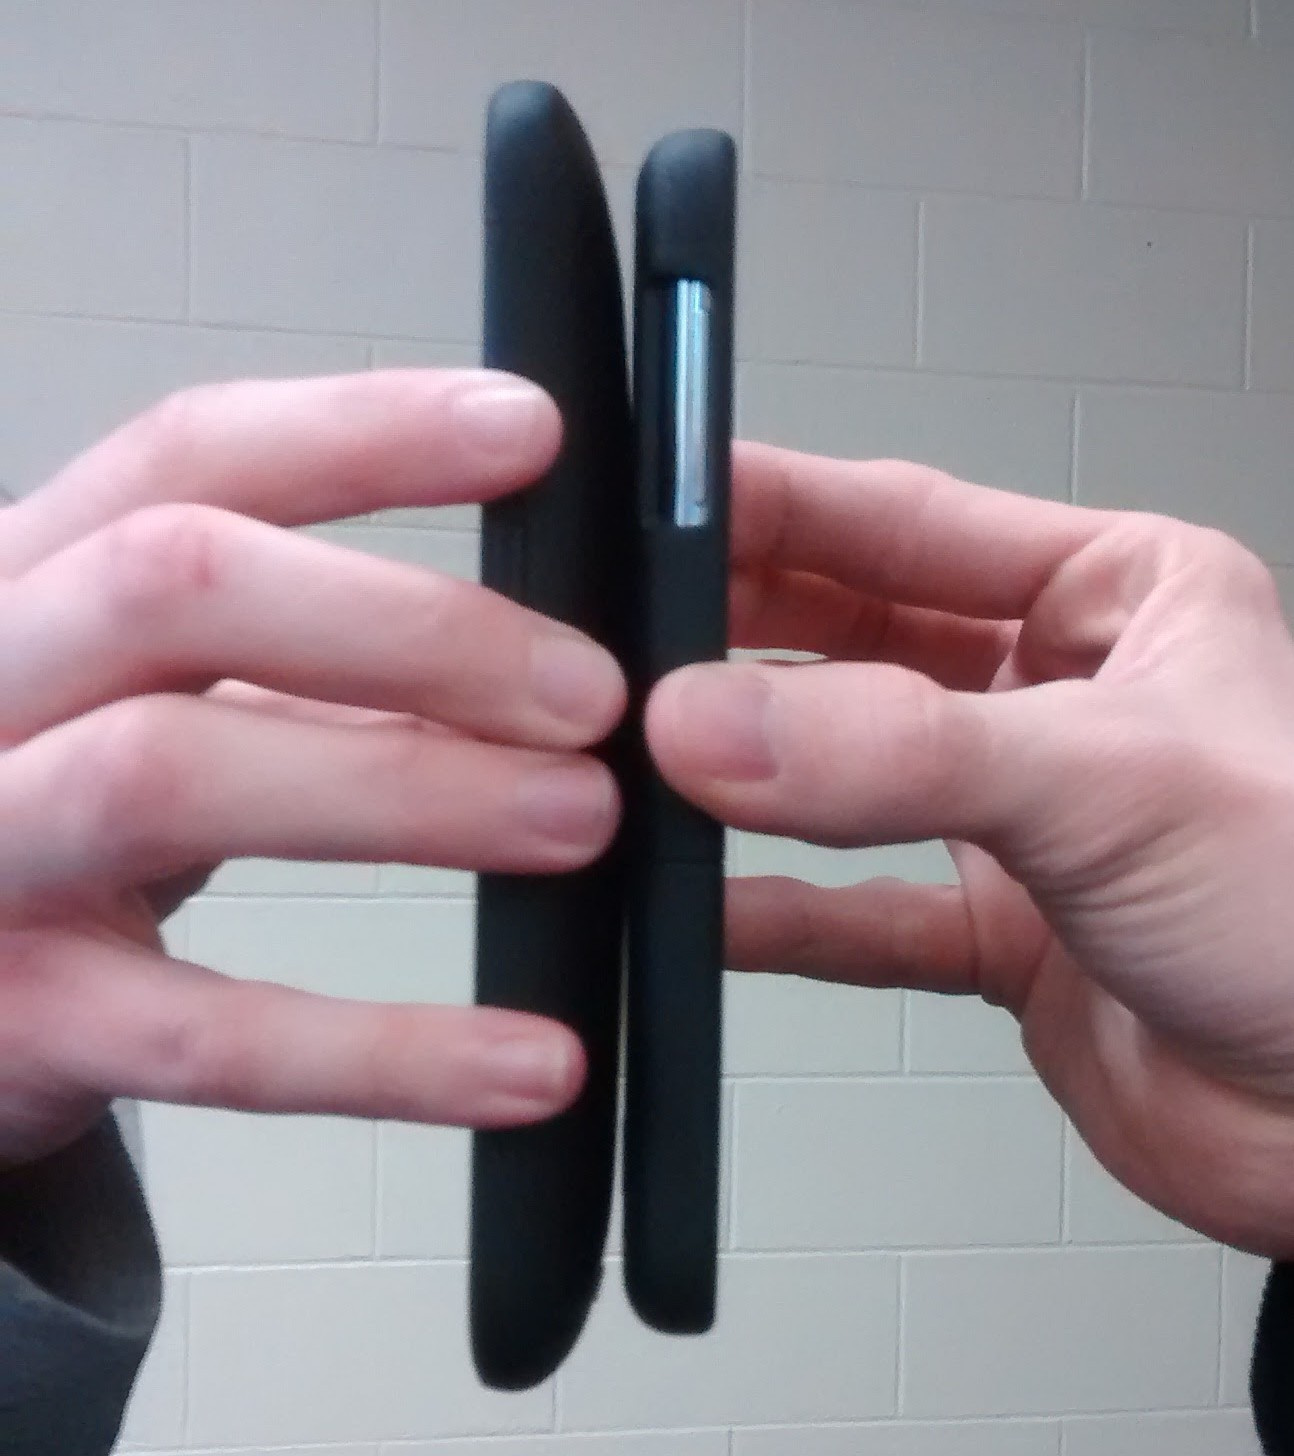
\includegraphics[width=\linewidth,height=0.3\textheight,keepaspectratio]{figures/peer.jpg}
        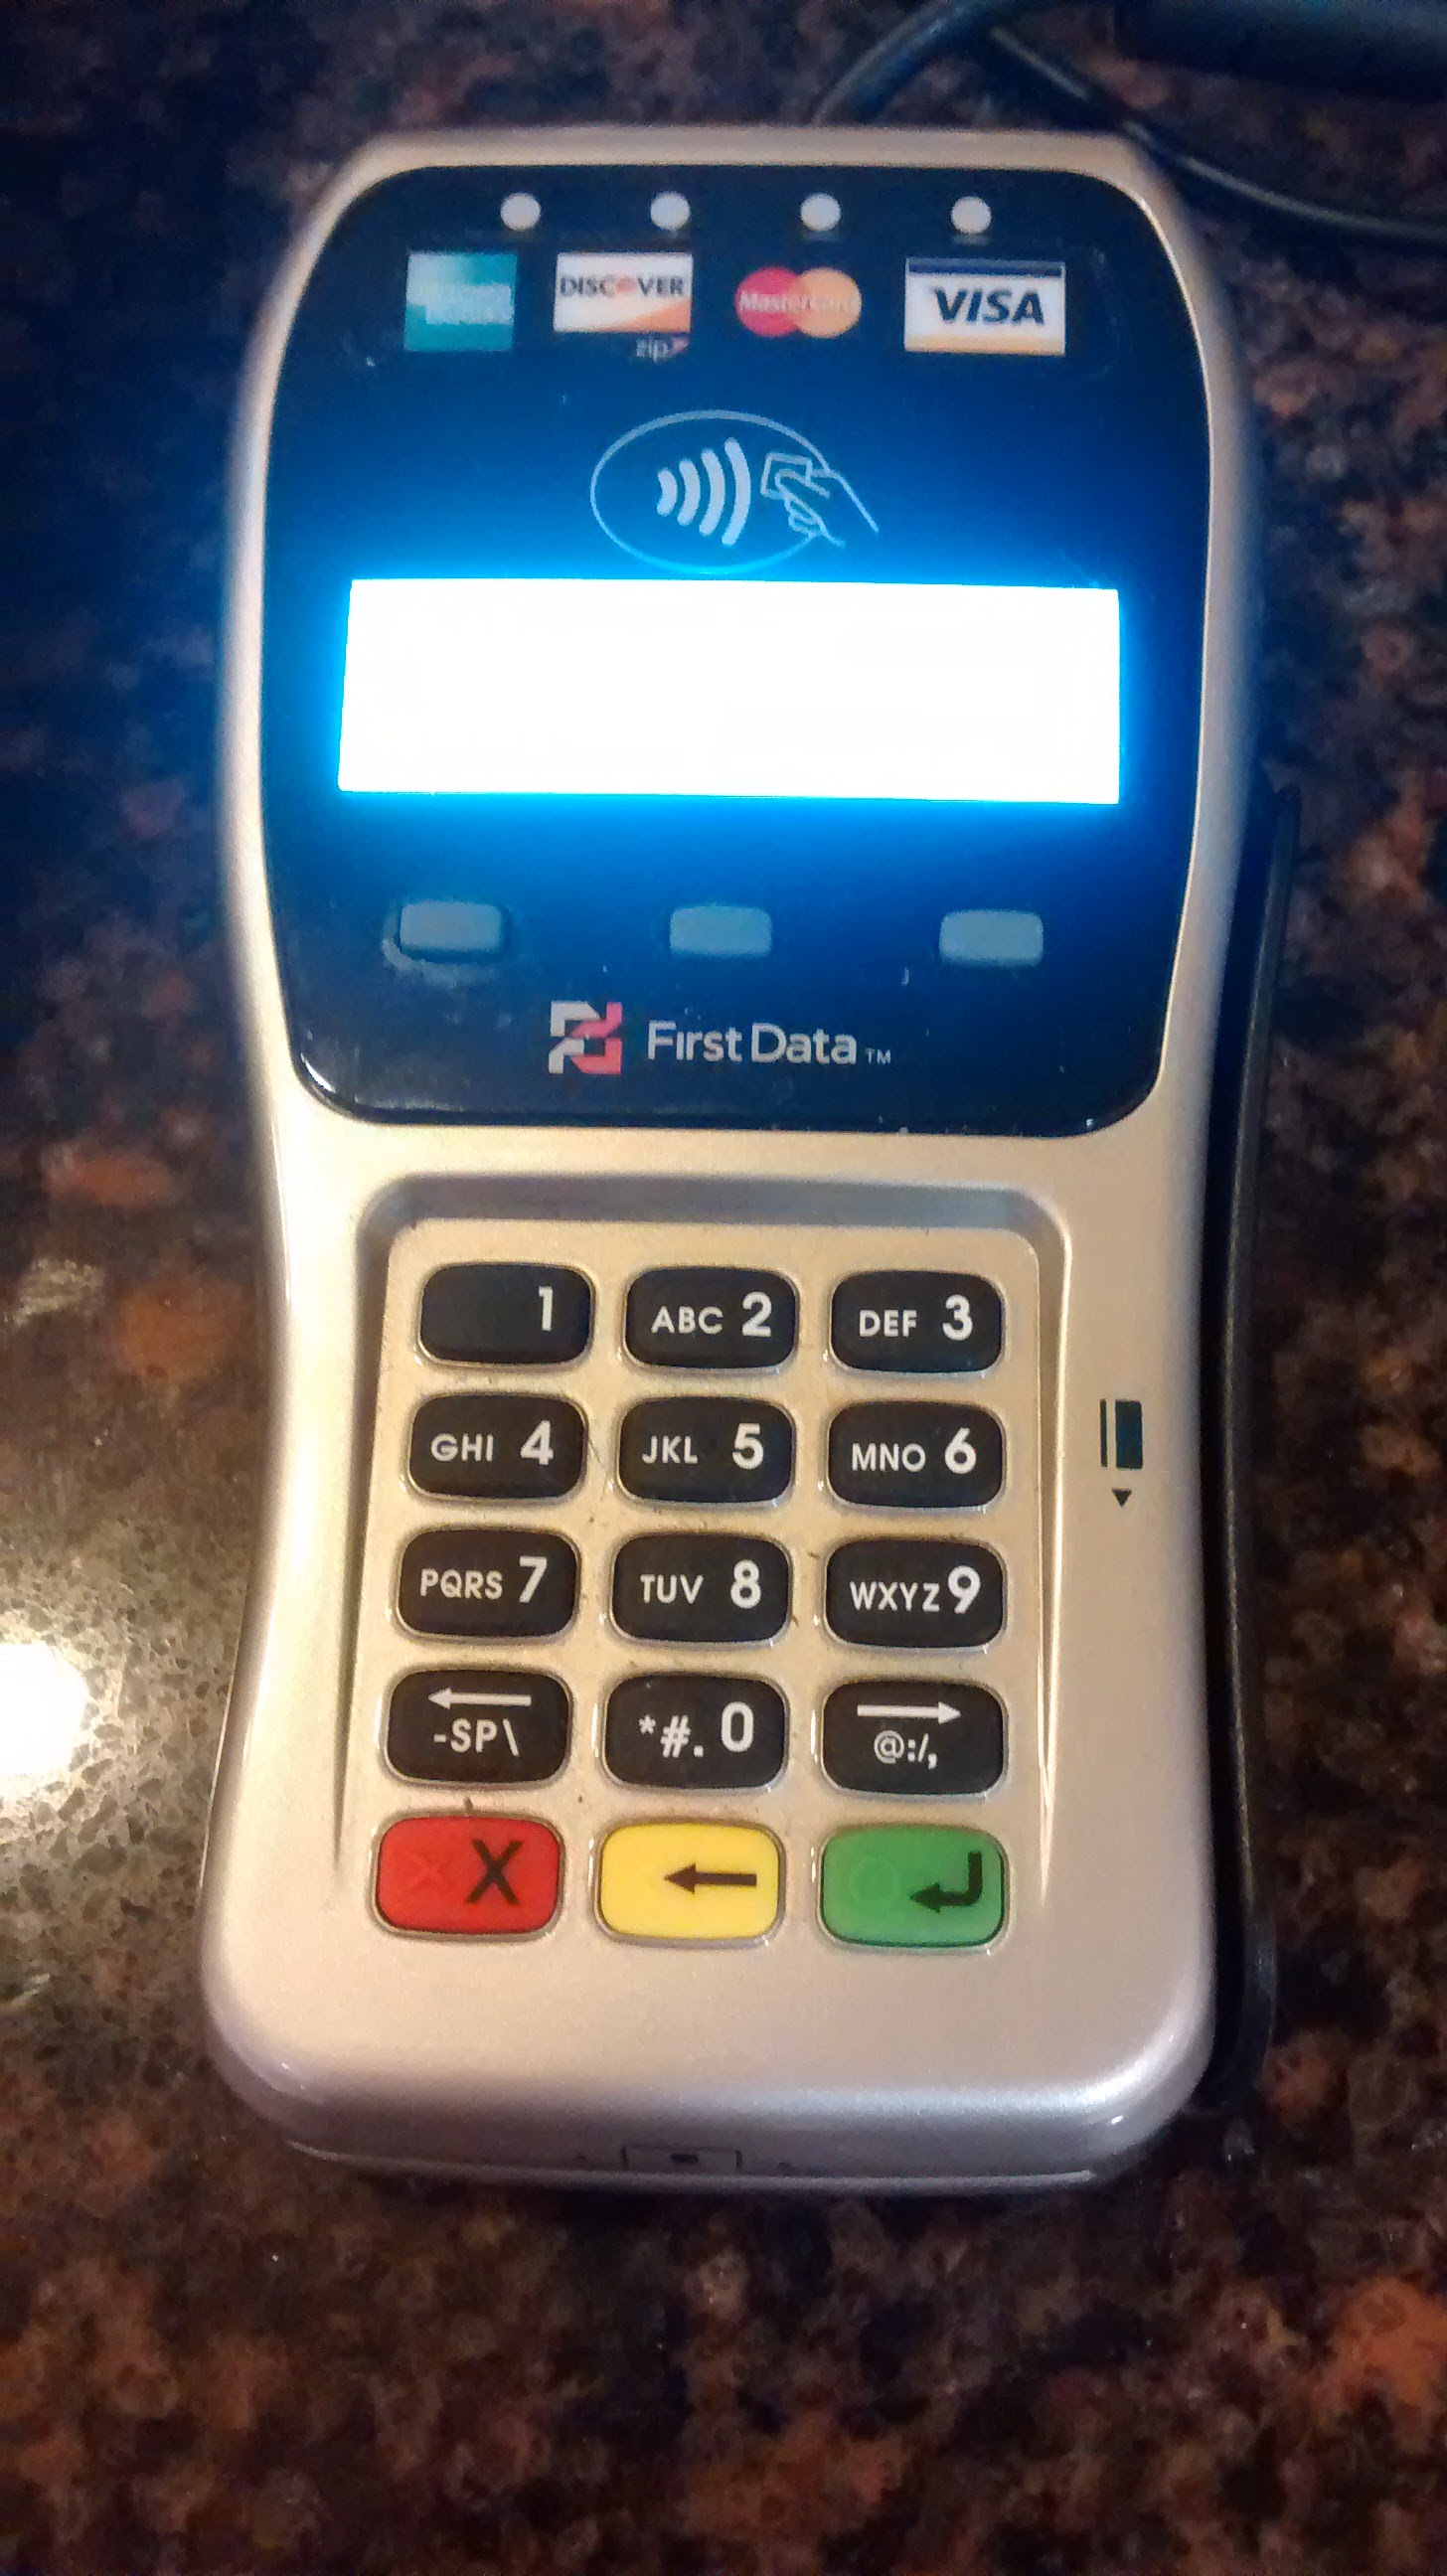
\includegraphics[width=\linewidth,height=0.3\textheight,keepaspectratio]{figures/higbies.jpg}
      \end{center}
    \end{block}
    \textref{Note: The communication standard used in UCard was not verified}
\end{frame}

\begin{frame}
\frametitle{Motivation}
  \begin{center}
    \begin{minipage}{.7\textwidth}
  	 \begin{block}{Questions about NFC}
        \begin{itemize}
  		    \item{What is NFC and how does it work?}
  		    \item{Is it secure and should I trust it?}
  		    \item{Is NFC the future?}
     		\end{itemize}
     \end{block}
    \end{minipage}
  \end{center}
\end{frame}

\begin{frame}
  \frametitle{Outline}
    \begin{center}\begin{minipage}{.9\textwidth}
        \tableofcontents[
          currentsection,
          sectionstyle=show/show,
          subsectionstyle=show/shaded/hide
        ]
    \end{minipage}\end{center}
 \end{frame}


\Fontix

%-------------------------------------------------------------------
%                           Section
\section{Background}
\begin{frame}
  \frametitle{Background}
    \begin{center}\begin{minipage}{.9\textwidth}
    \tableofcontents[currentsubsection, hideothersubsections, sectionstyle=show/shaded]
    \end{minipage}\end{center}
\end{frame}
%
%-------------------------------------------------------------------


\subsection{Elements of HF RFID: Tags \& Readers}
\begin{frame}
  \frametitle{Introduction to HF-RFID}
    \begin{center}\begin{minipage}{.9\textwidth}
      \begin{itemize}
        \item{NFC is built using elements of \textit{high-frequency radio frequency identification} (HF RFID)}\newline

        \begin{minipage}{.9\textwidth}\centering
          \vspace{5mm}
          \includegraphics<1>[width=\linewidth,height=0.2\textheight,keepaspectratio]{figures/rfid.png}
          \includegraphics<2->[width=\linewidth,height=0.2\textheight,keepaspectratio]{figures/rfidFade.png}
        \end{minipage}
        \vspace{5mm}
        \item<3->{Range depends on frequency, size of antenna, power, and interference}
        \item<4->{Communication happens between tags and readers}
      \end{itemize}
    \end{minipage}\end{center}
\end{frame}


\begin{frame}
\frametitle{Tags \& Readers}

  \begin{columns}[T]
    \begin{column}{.5\textwidth}\centering
        \vspace{3mm}
        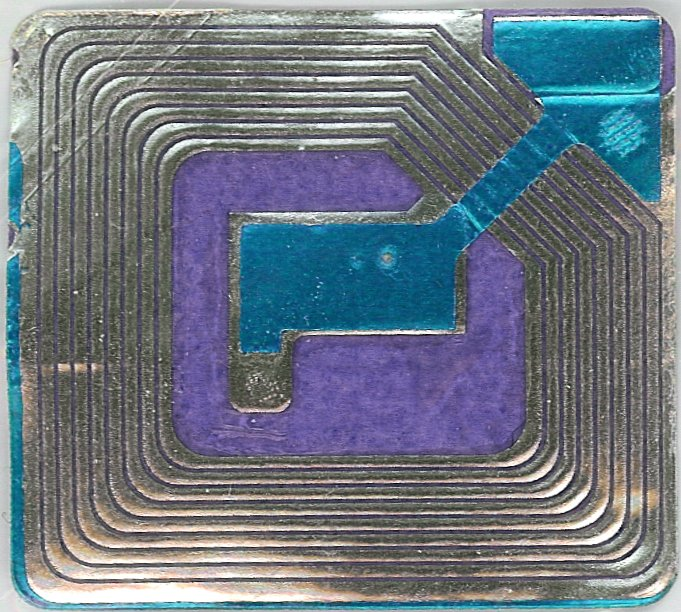
\includegraphics[width=\linewidth,height=0.2\textheight,keepaspectratio]{figures/wikimediatagWide.jpg}
    \end{column}
    \begin{column}{.5\textwidth}
        \begin{block}{Tag}
          \begin{itemize}
              \item{A tiny circuit with an antenna coil}
              \pause
              \item{Stores limited information}
              \pause
              \item{Can be powered or passive}
              \pause
              \item{Passive tags are smallest and cheapest}
              \pause
            \end{itemize}
          \end{block}
    \end{column}
  \end{columns}

  \begin{columns}[T]
    \begin{column}{.5\textwidth}\centering
        \vspace{3mm}
        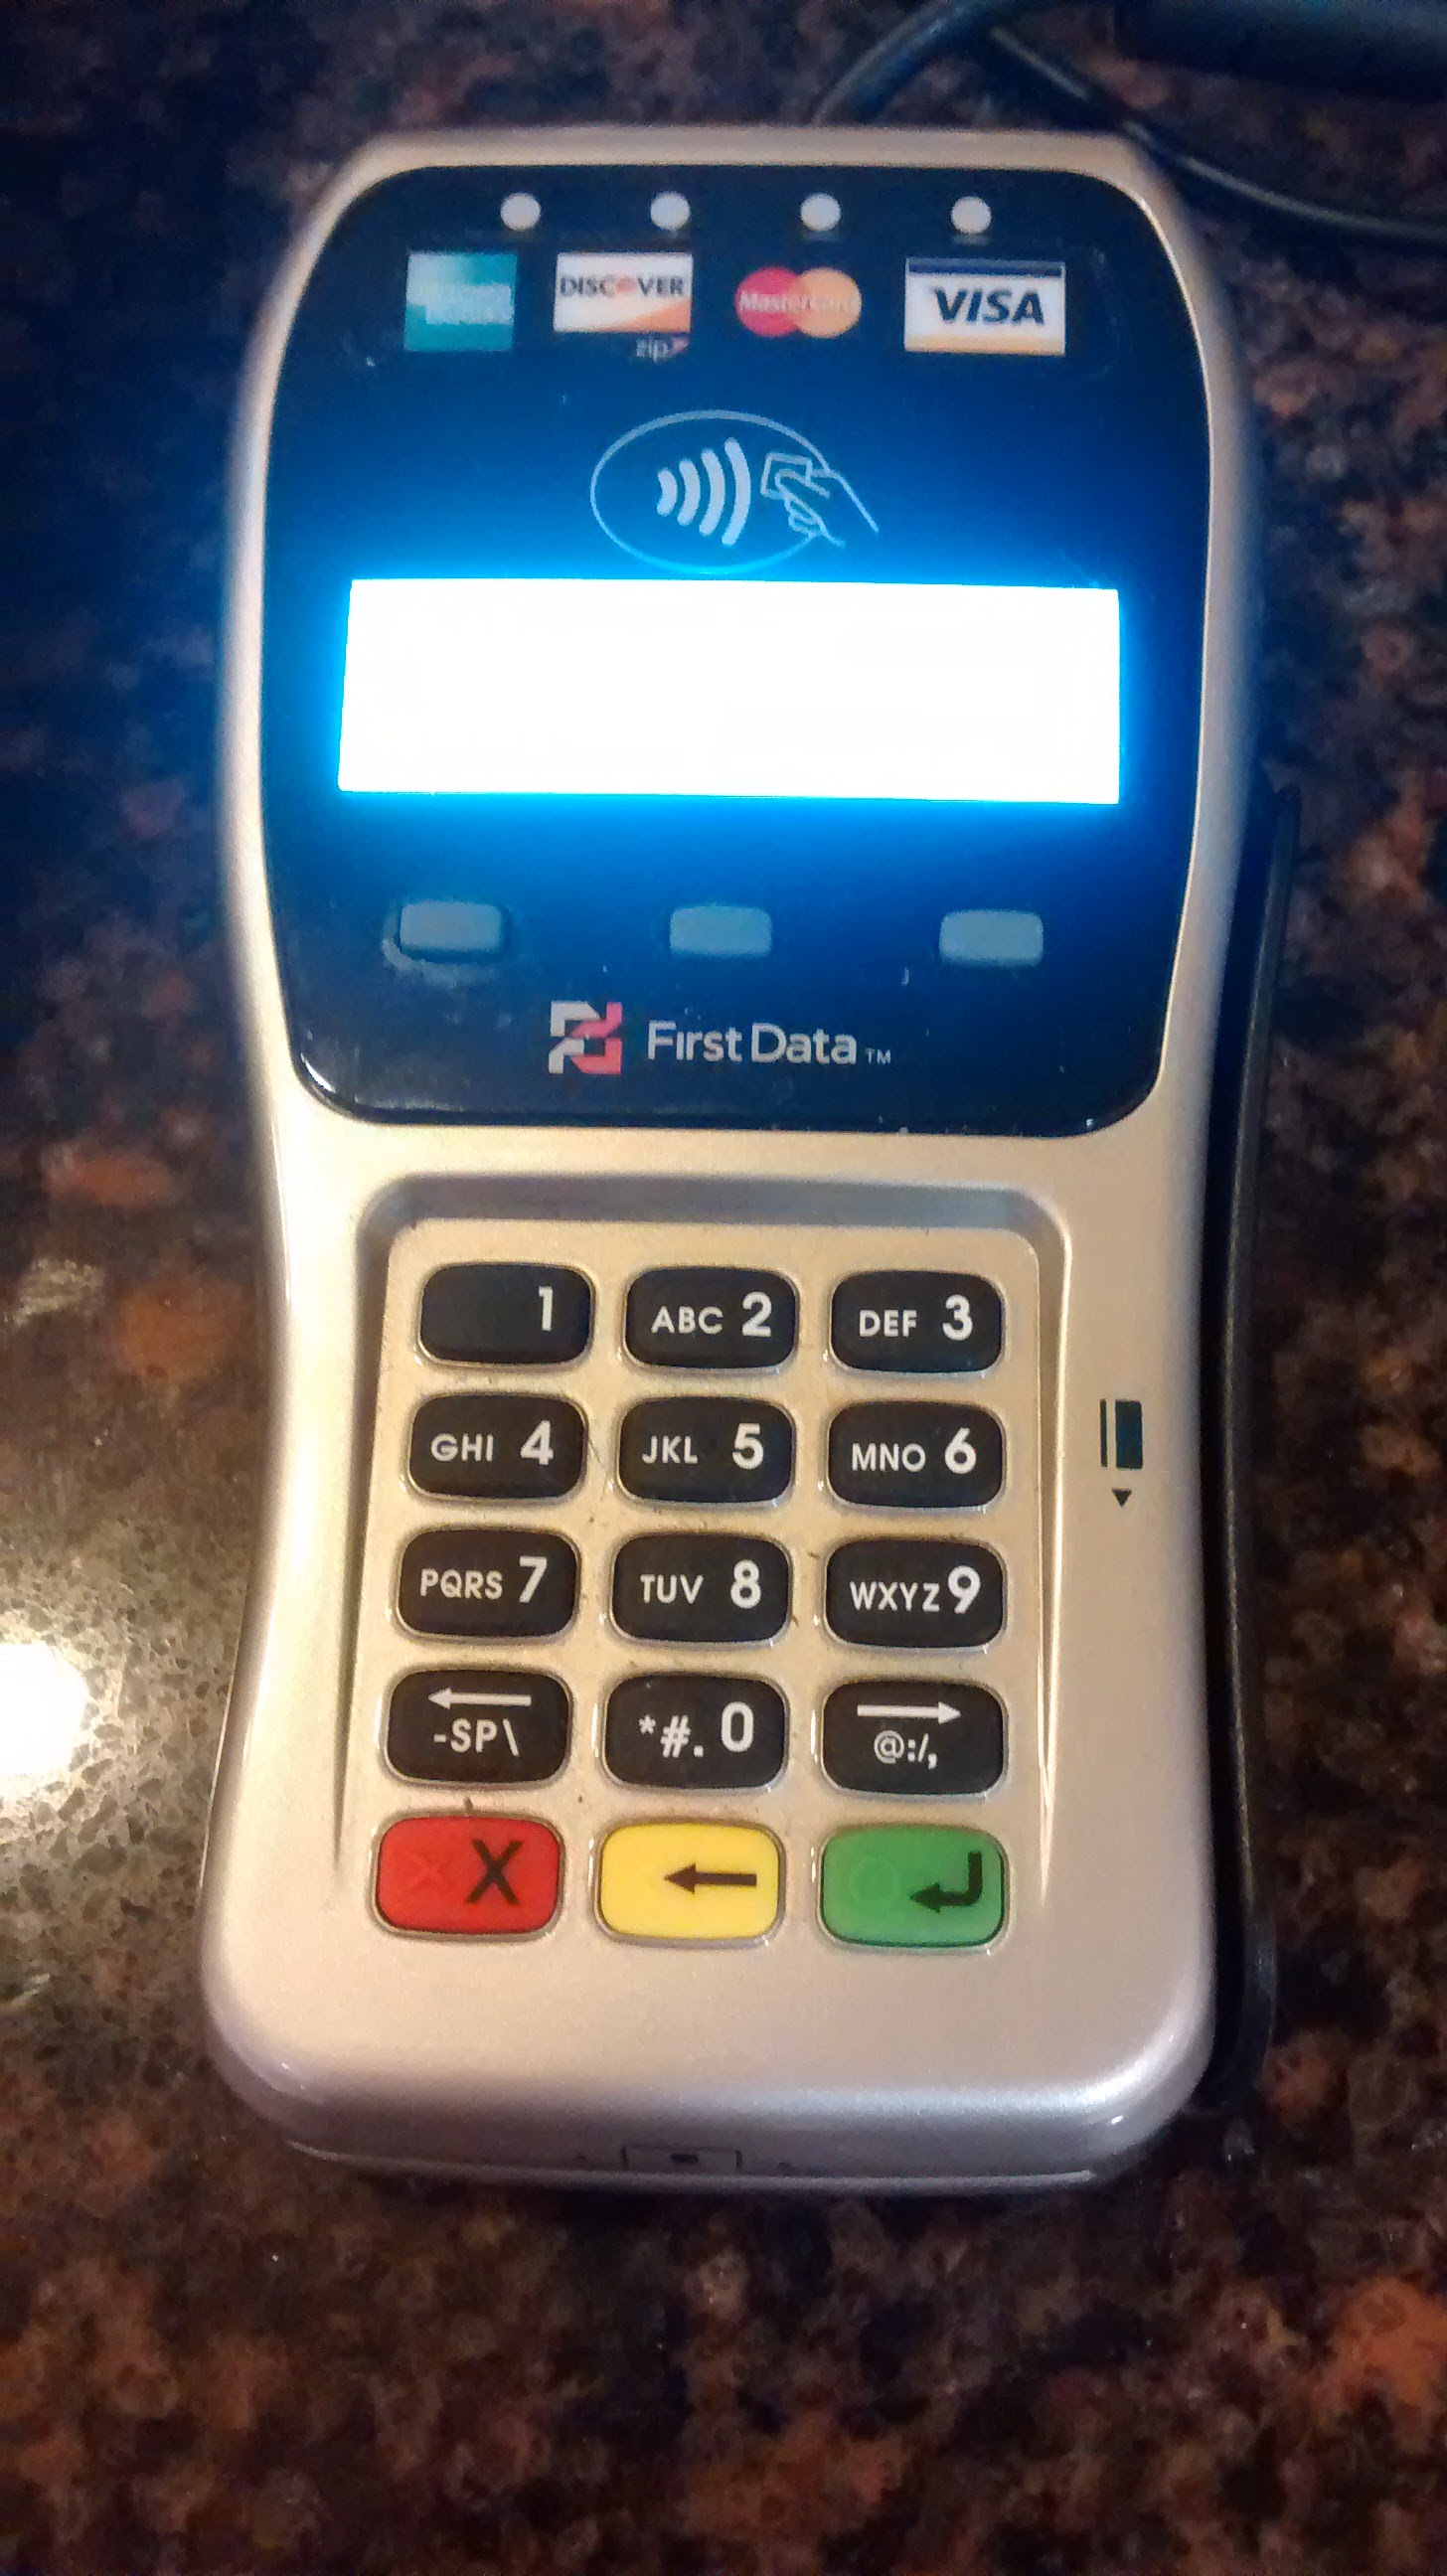
\includegraphics[width=\linewidth,height=0.2\textheight,keepaspectratio]{figures/higbies.jpg}
    \end{column}
    \begin{column}{.5\textwidth}
      \begin{block}{Reader}
	       \begin{itemize}
          \item{Reader emits electricity using an antenna coil}
          \pause
          \item{Initiates communication}
         \end{itemize}
       \end{block}
    \end{column}
  \end{columns}
\end{frame}



\begin{frame}
\frametitle{Contactless Communication}
  \begin{center}\begin{minipage}{.9\textwidth}
  \vspace{4mm}
  \begin{columns}[T]
    \begin{column}{.5\textwidth}
      \begin{block}{}
        \begin{center}
          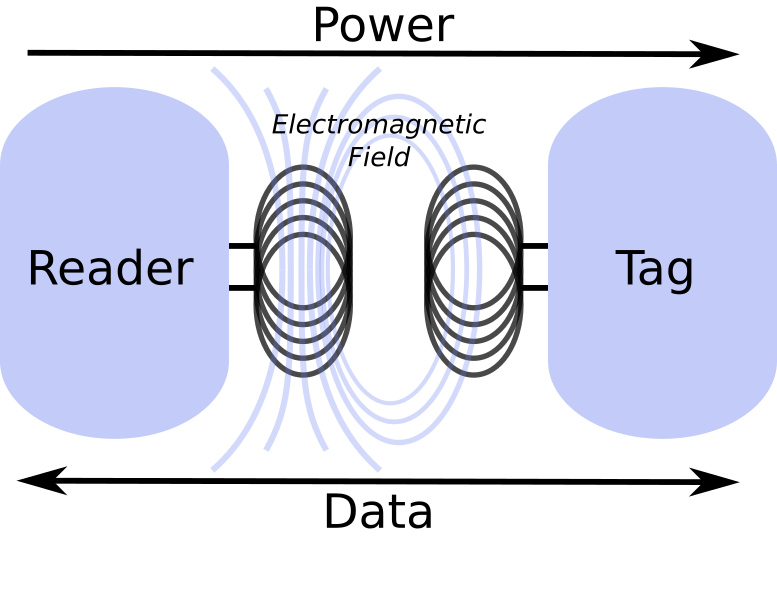
\includegraphics[width=0.4\paperwidth]{figures/emitterAndTag.png}
        \end{center}
      \end{block}
    \end{column}
    \begin{column}{.5\textwidth}
      \vspace{4mm}
     \begin{block}{HF-RFID Communication}
		\begin{enumerate}
        \pause
		    \item{Reader emits electricity}
        \pause
		    \item{Tag is activated by induced power}
        \pause
      	\item{Reader runs discovery protocol, selecting tag by unique ID}
        \pause
      	\item{Communication ensues}
   		\end{enumerate}
    \end{block}
%    \pause
%    \begin{block}{Features}
%		  \begin{itemize}
%        	\item{Quick setup}
%        	\item{Line of sight not required}
%   		\end{itemize}
%    \end{block}
    \end{column}
  \end{columns}
  \end{minipage}\end{center}
\end{frame}


%\subsection{Physics: Electromagnetic Induction}
%\begin{frame}
%  \frametitle{Physics: Electromagnetic Induction}
%\end{frame}
%%%%reset slide%%%
%\begin{frame}
%\frametitle{\ul{Physics:} Electromagnetic Induction}
%  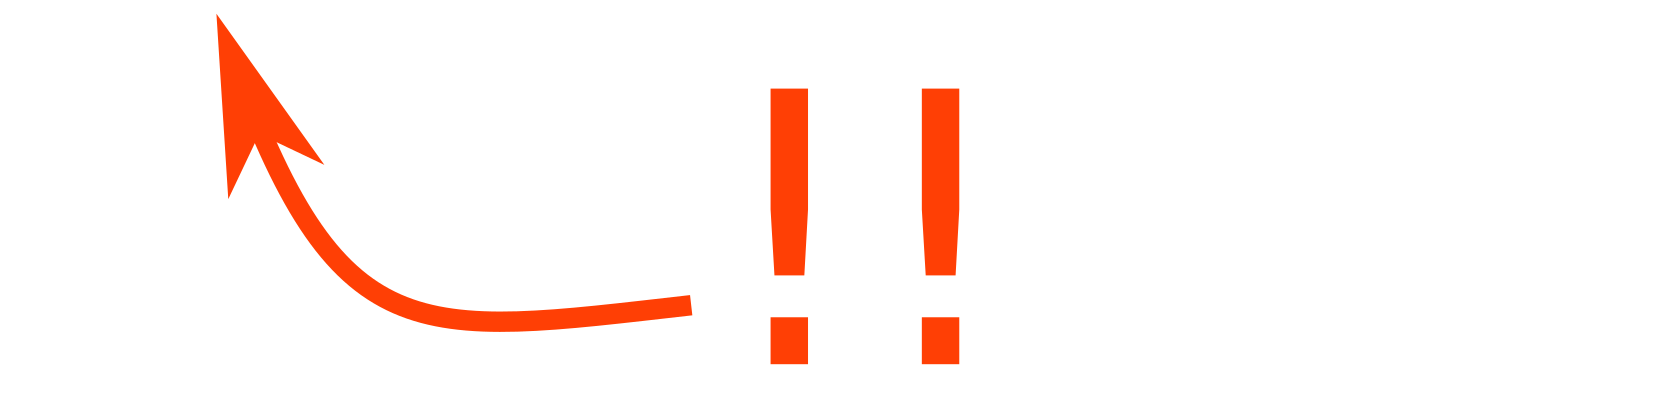
\includegraphics[scale=.5]{figures/arrow.png}
%  \begin{center}\begin{minipage}{.9\textwidth}
%     \begin{block}{Tom, this is a computer science presentation, \newline not physics...}
%     	%But its pretty neat stuff.
%     \end{block}
%  \end{minipage}\end{center}
%\end{frame}
%%%%reset slide%%%
%\begin{frame}
%\frametitle{Physics: Electromagnetic Induction}
%  \begin{center}\begin{minipage}{.9\textwidth}
%    %To show very quickly
%     \begin{block}{But its physics, and scary...}
%     \end{block}
%  \end{minipage}\end{center}
%\end{frame}
%%%%reset slide%%%
%\begin{frame}
%\frametitle{Physics: Electromagnetic Induction}
%  \begin{center}\begin{minipage}{.9\textwidth}
%  NFC and RFID uses \textit{electromagnetic induction}, the same technology used in power transformers \newline
%  \begin{columns}[T]
%  \begin{column}{.5\textwidth}
%    \begin{block}{}\begin{center}
%      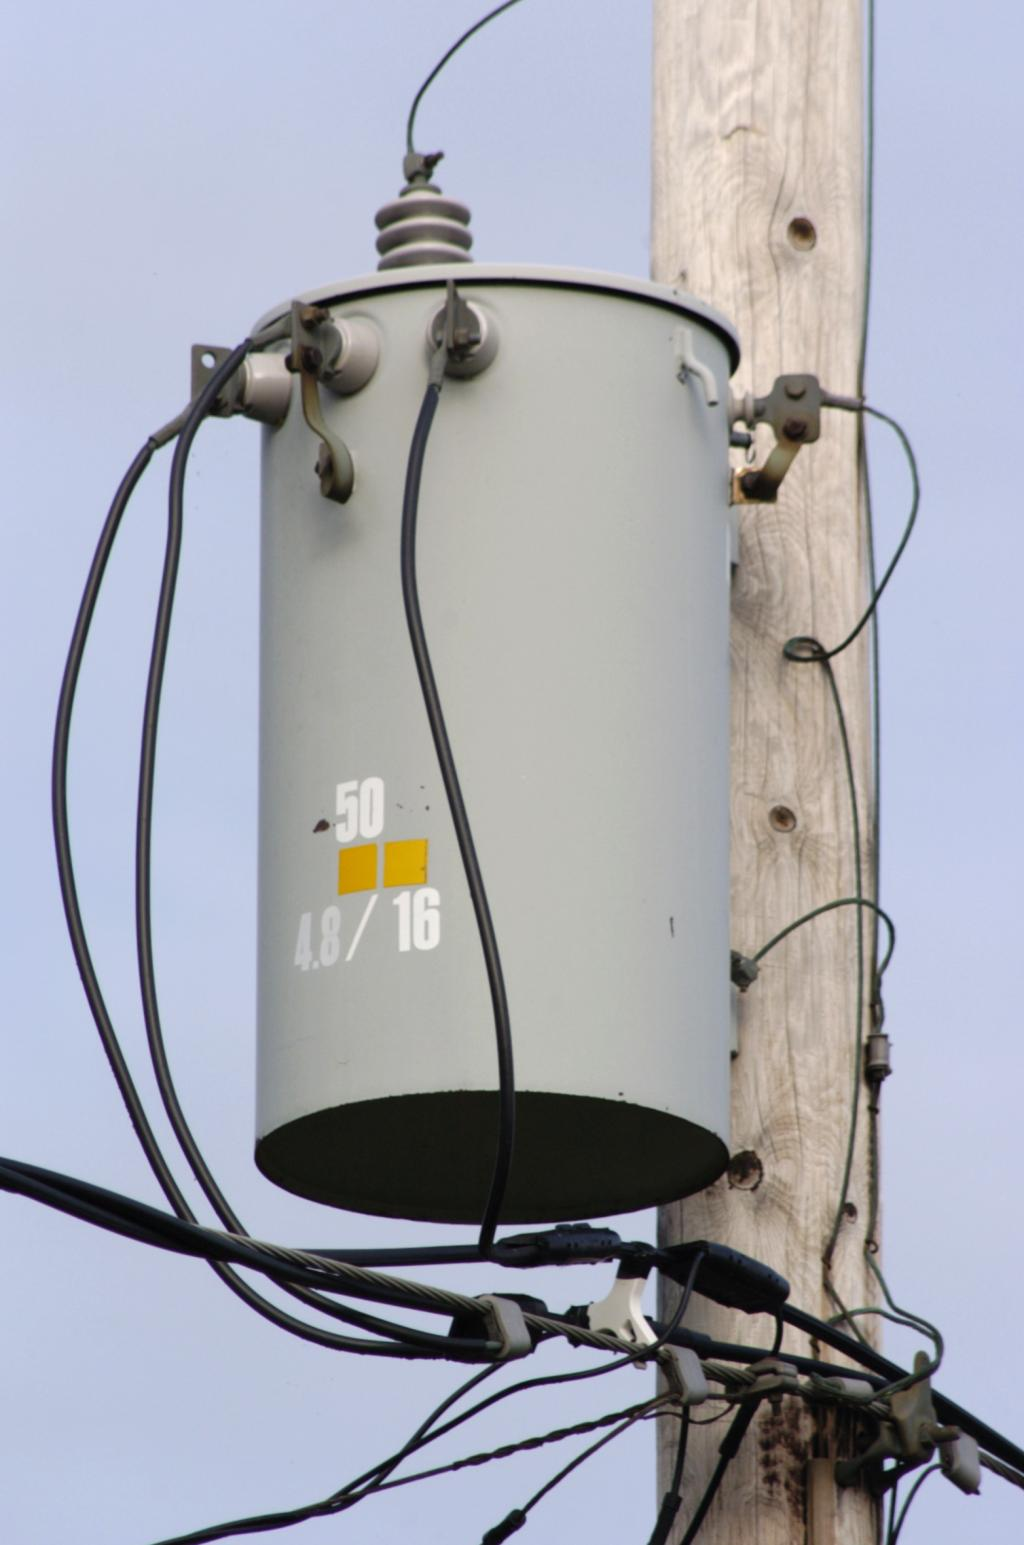
\includegraphics[width=0.2\paperwidth]{figures/Polemount-singlephase-closeup.jpg}
%    \end{center}\end{block}
%  \end{column}
%    \begin{column}{.5\textwidth}
%      \begin{block}{}\begin{center}
%        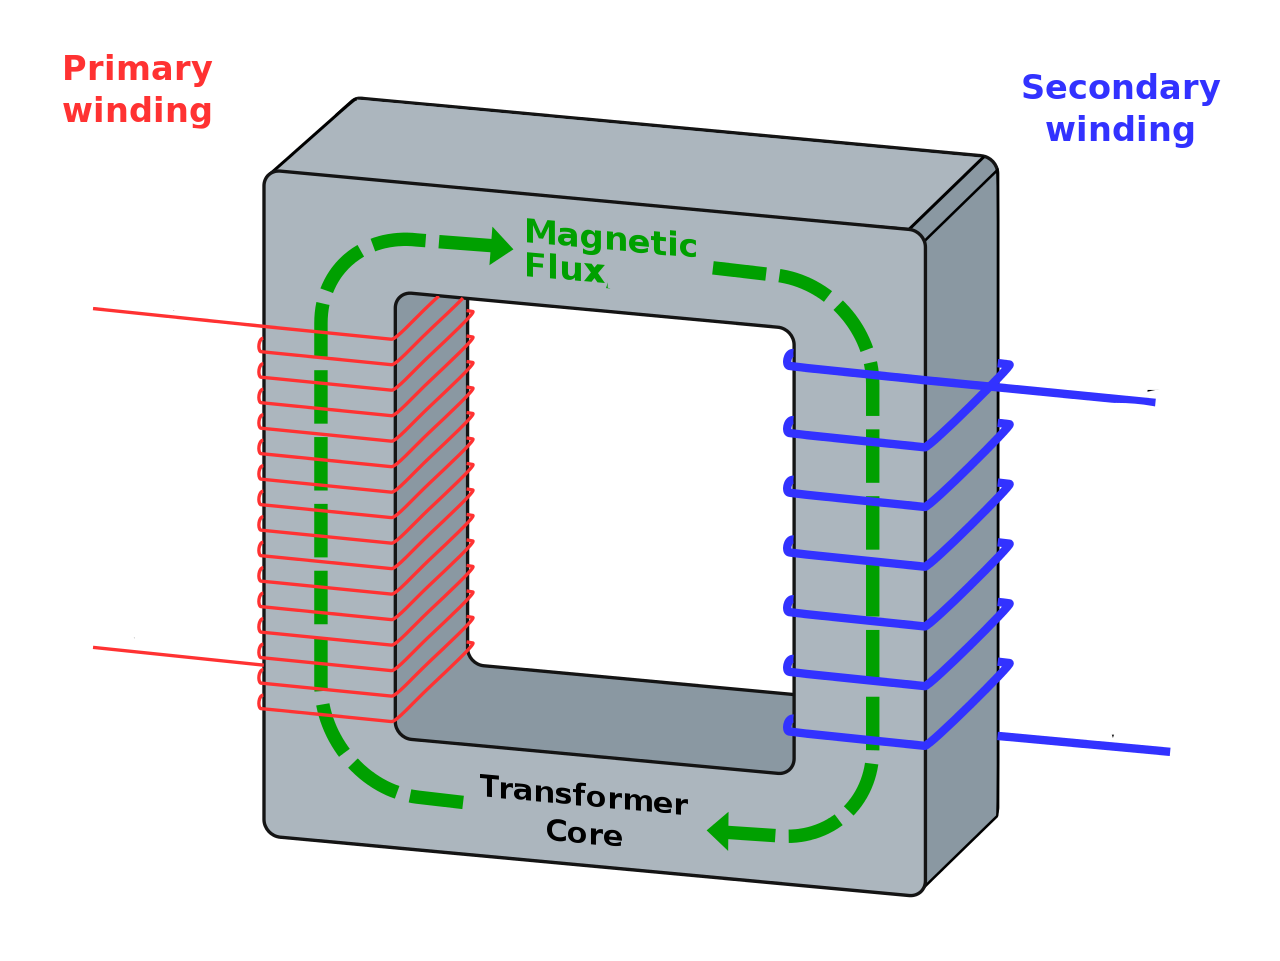
\includegraphics[width=0.4\paperwidth]{figures/solidcore.png}
%      \end{center}\end{block}
%    \end{column}
%  \end{columns}
%  \end{minipage}\end{center}
%  \textref{Images originate from "Transformers" page on Wikipedia}
%\end{frame}
%%%%reset slide%%%
%\begin{frame}
%\frametitle{Physics: Electromagnetic Induction}
%  \begin{center}\begin{minipage}{.9\textwidth}
%     \begin{block}{End physics interlude.}
%     \end{block}
%  \end{minipage}\end{center}
%\end{frame}



\subsection{NFC on Mobile Phones}

\begin{frame}
\frametitle{NFC on Mobile Phones}
  \begin{center}
  \begin{minipage}{.7\textwidth}
  \begin{block}{NFC extends HF RFID:}
		\begin{enumerate}
		  \item{Phones can act as readers}
		  \item{Phones can emulate tags}
      \item{Phones can communicate peer-to-peer}
   	\end{enumerate}
  \end{block}
  \end{minipage}
  \end{center}
\end{frame}

\begin{frame}
\frametitle{NFC on Mobile Phones}
  \begin{center}
  \begin{minipage}{.7\textwidth}
  \begin{block}{\circled{1}~~Phones can act as readers}\centering
      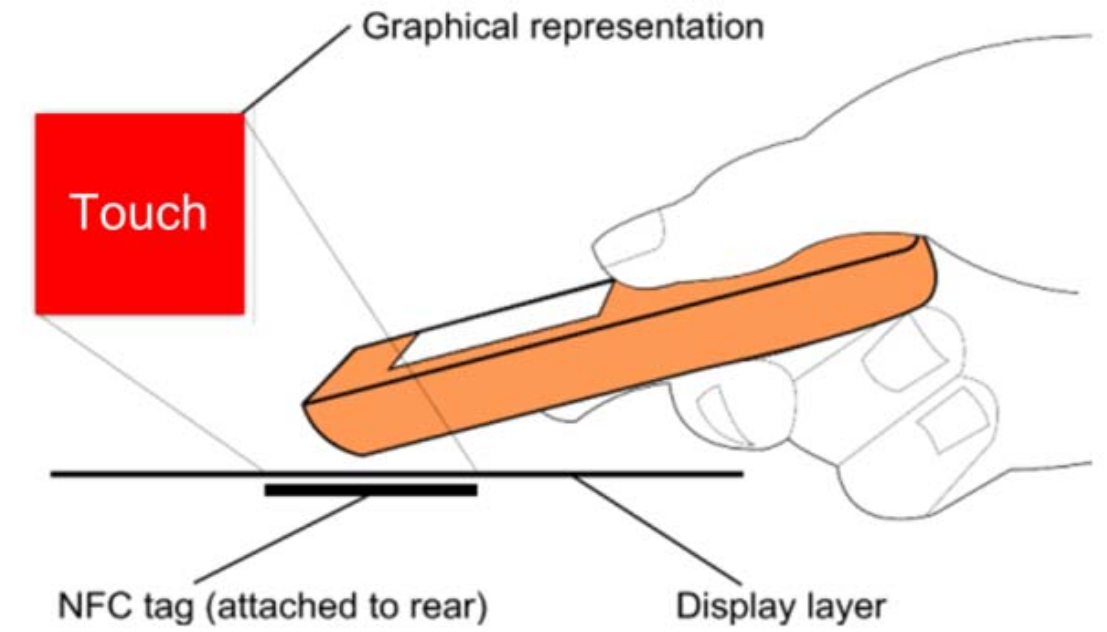
\includegraphics[width=\linewidth,height=0.2\textheight,keepaspectratio]{figures/hardy.png}
      \begin{itemize}
  		  \item{Phones read NFC tags as if they were QR codes}
        \pause
  		  \item{Touching a tag mounted to a map could bring up tourist information}
        \pause
        \item{Research into using tags as a user interface}
     	\end{itemize}
  \end{block}
  \end{minipage}
  \end{center}
  \textref{Image from Hardy 2010}
\end{frame}

\begin{frame}
\frametitle{NFC on Mobile Phones}
  \begin{center}
  \begin{minipage}{.7\textwidth}
  \begin{block}{\circled{2}~~Phones can emulate tags}\centering
      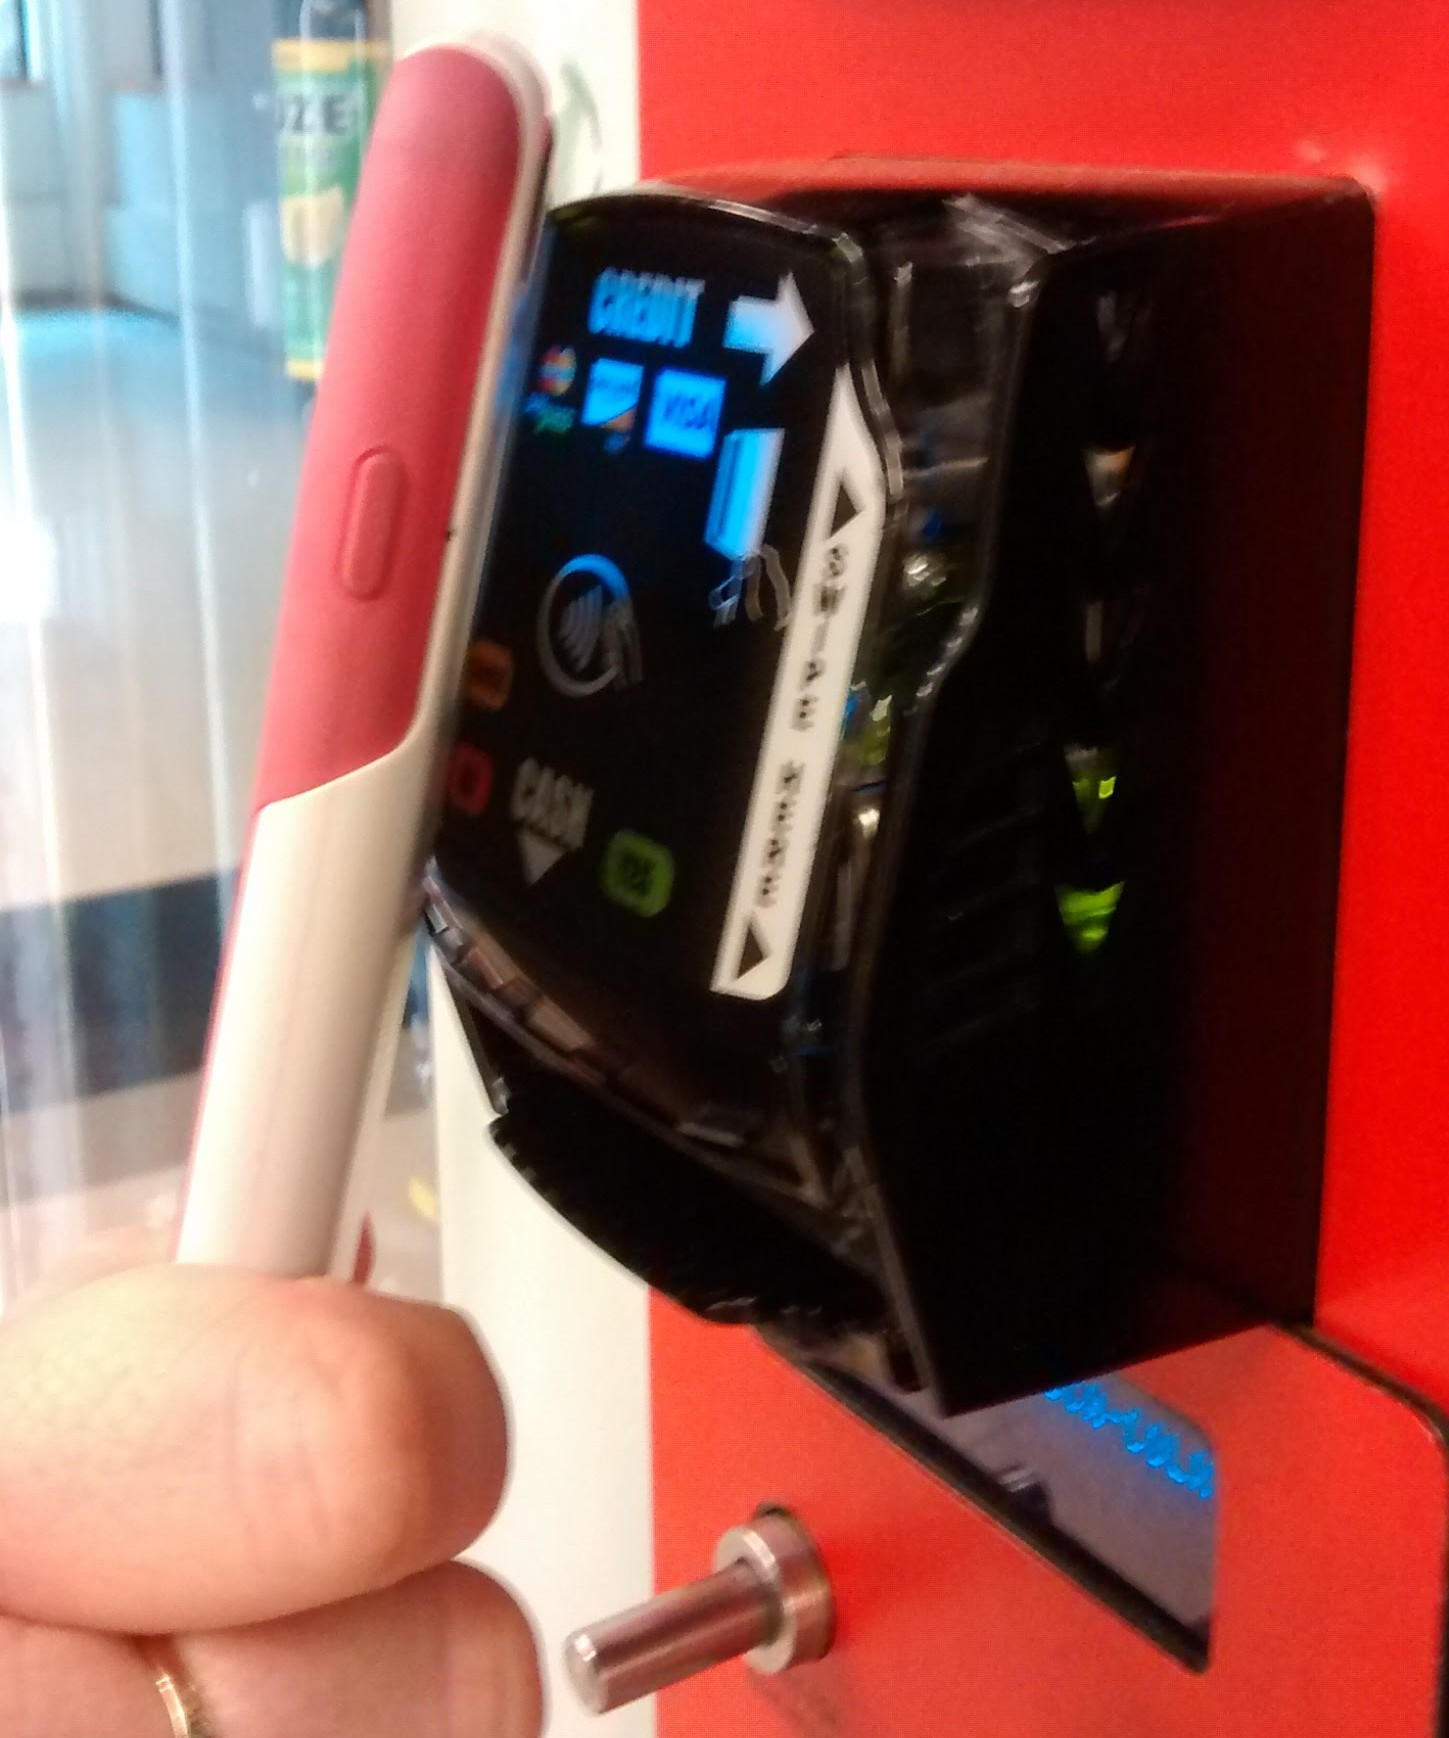
\includegraphics[width=\linewidth,height=0.2\textheight,keepaspectratio]{figures/ApplePay.jpg}
      \begin{itemize}
  		  \item{Phones acts as if it were a passive tag}
        \pause
  		  \item{A possibility for payments or ticketing applications}
     	\end{itemize}
  \end{block}
  \end{minipage}
  \end{center}
  \textref{Image Note: Thank you Angela}
\end{frame}

\begin{frame}
\frametitle{Phones can communicate peer-to-peer}
  \begin{center}
  \begin{minipage}{.7\textwidth}
  \begin{block}{\circled{3}~~Phones can communicate as peers}\centering
      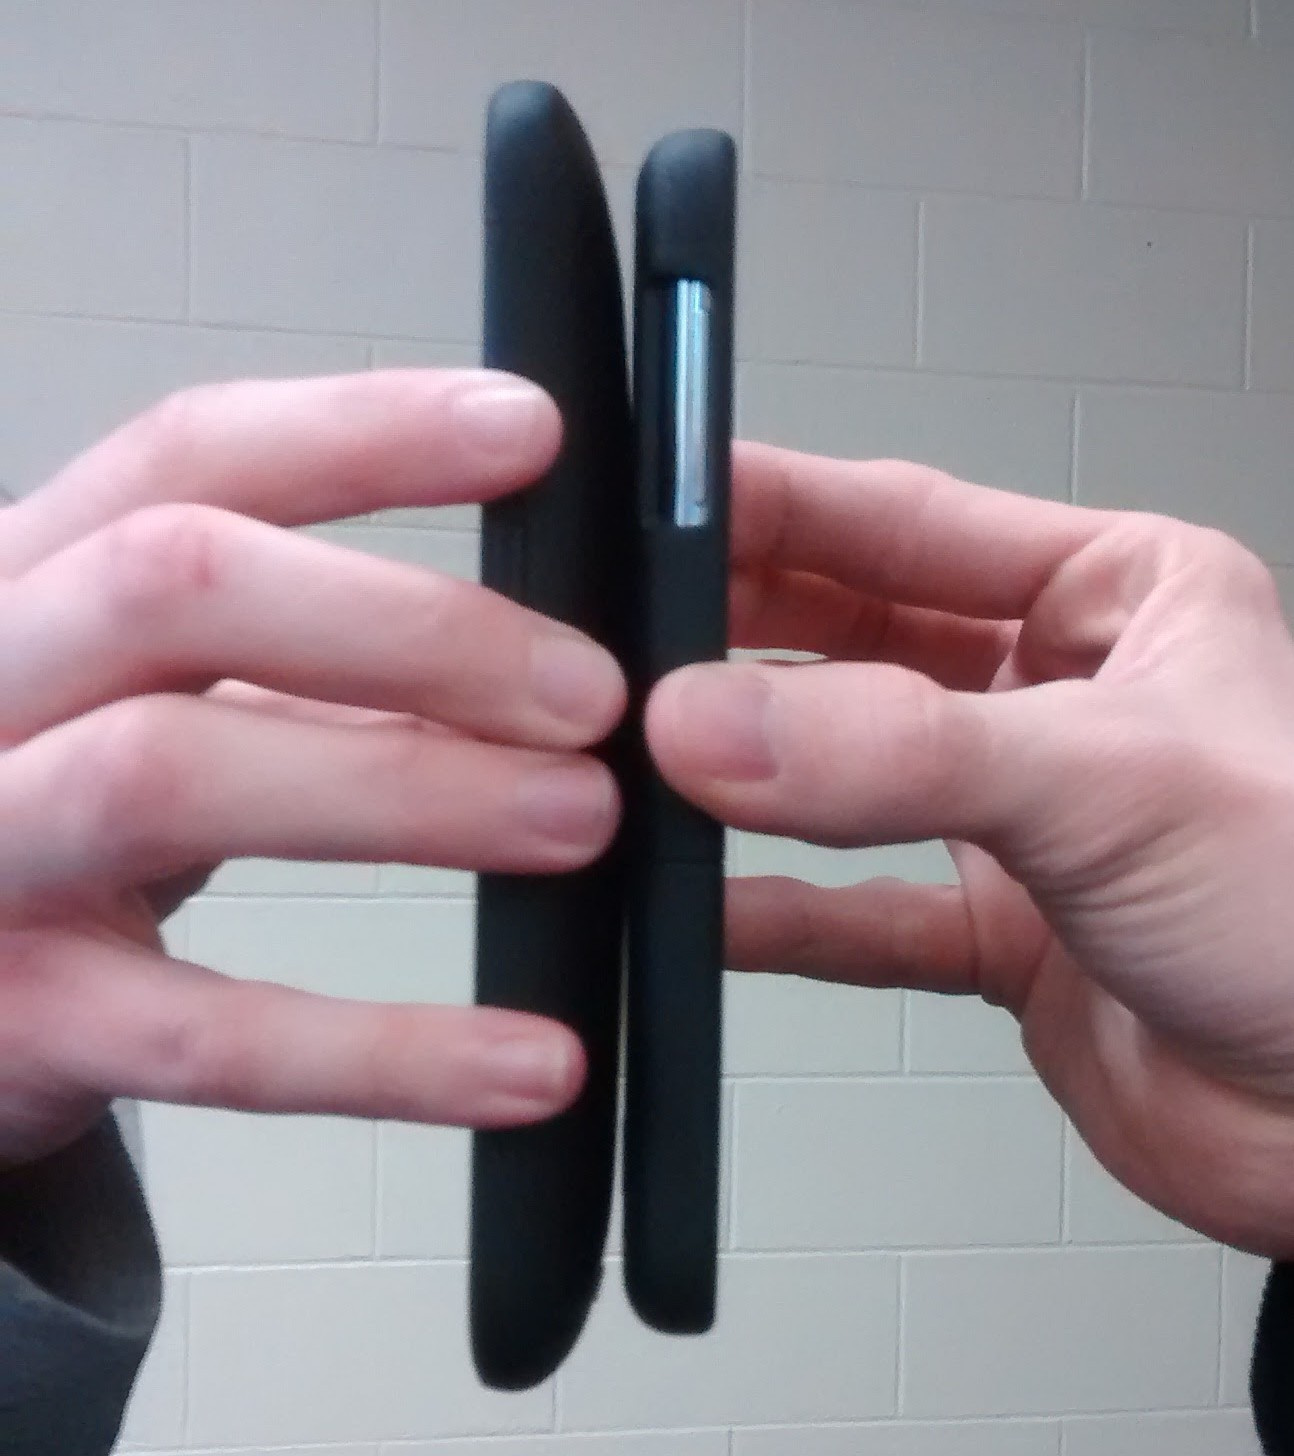
\includegraphics[width=\linewidth,height=0.2\textheight,keepaspectratio]{figures/peer.jpg}
      \begin{itemize}
  		  \item{Phones take turns switching between reader and tag-emulation mode}
        \pause
  		  \item{Highest NFC communication throughput}
        \pause
  		  \item{Can be used as a basis for stronger security or file transfers}
     	\end{itemize}
  \end{block}
  \end{minipage}
  \end{center}
  \textref{Image Note: Thank you Jacob and Maggie}
\end{frame}


\subsection{Security for NFC}
\begin{frame}
\frametitle{Security for NFC}
  \begin{center}
  \begin{minipage}{.7\textwidth}
  \begin{block}{NFC is not inherently secure}
    \begin{enumerate}
      \item{NFC's limited range makes attacks difficult, but not impossible}
      \item{Features like confidentiality, integrity, and authentication need to be implemented as an extension of NFC}
    \end{enumerate}
  \end{block}
  \end{minipage}
  \end{center}
\end{frame}

%-------------------------------------------------------------------
%                           Section
\section{Contactless Credit Cards}
\subsection{Current Credit Card Protocol}
\begin{frame}
  \frametitle{Contactless Credit Cards}
    \begin{center}\begin{minipage}{.9\textwidth}
    \tableofcontents[currentsubsection, hideothersubsections, sectionstyle=show/shaded]
    \end{minipage}\end{center}
\end{frame}
%
%-------------------------------------------------------------------
\begin{frame}
\frametitle{Contactless Credit Cards}
  \begin{center}
  \begin{minipage}{.9\textwidth}
  \begin{block}{Contactless Credit Cards}
    \begin{itemize}
      \item{Some credit cards contain passive NFC tags}
      \pause
      \item{We focus on Jensen, Gouda, and Qiu's [1] work on securing such cards in this section}
      \pause
      \item{Security solutions must be computationally inexpensive to run on passive tags}
    \end{itemize}
  \end{block}
  \end{minipage}
  \end{center}
\end{frame}

\begin{frame}
\frametitle{Limited Security via iCVV}
  \begin{center}
  \begin{minipage}{.9\textwidth}
  \begin{block}{Contactless Credit Cards}
    \begin{itemize}
      \item{Card generates a pseudo-random \textit{Dynamic Card Validation Value} (iCVV) for each transaction}
      %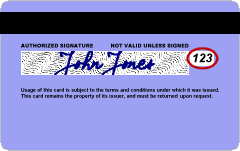
\includegraphics[width=\linewidth,height=0.2\textheight,keepaspectratio]{figures/CVC2SampleVisaNew.png}
      \pause
      \item{The iCVV is sent to point of sale and then validated by bank}
    \end{itemize}
  \end{block}
  \end{minipage}
  \end{center}
  %\textref{Image and background information taken from "Card security code" page on Wikipedia}
\end{frame}

\begin{frame}
\frametitle{Current Credit Protocol}\centering
  \includegraphics<1>[scale=.5]{figures/CCcurrent0.png}
  \includegraphics<2>[scale=.5]{figures/CCcurrent1.png}
  \includegraphics<3>[scale=.5]{figures/CCcurrent2.png}
  \includegraphics<4>[scale=.5]{figures/CCcurrent3.png}
  \includegraphics<5>[scale=.5]{figures/CCcurrent4.png}
  \newline\vspace{3mm}
    \begin{minipage}[t][5mm][t]{.7\textwidth}
      \only<1>{
        \begin{block}{Security depends upon}
          \begin{itemize}
            \item{Each transaction's card generated iCVV}
            \item{The limited range of NFC}
          \end{itemize}
        \end{block}
      }
      \only<2>{
        \begin{block}{Solicitation}
          \begin{itemize}
            \item{Point of Sale and Credit card exchange static messages}
            \item{For example, card may identify itself as \texttt{VISA CREDIT}}
          \end{itemize}
        \end{block}
      }
      \only<3>{
        \begin{block}{Card Information}
          \begin{itemize}
            \item{Credit card transmits card information, including:\newline
            \textbf{\textcolor{uipaleblue}{card number, expiration, bank name, and iCVV}}}
            \item{Unfortunately, this transmission is in plain text}
          \end{itemize}
        \end{block}
      }
      \only<4>{
        \begin{block}{Charge request}
          \begin{itemize}
            \item{Card number, expiration, and iCVV are sent to the indicated bank}
          \end{itemize}
        \end{block}
      }
      \only<5>{
        \begin{block}{Authorization}
          \begin{itemize}
            \item{Bank verifies transaction by checking iCVV, location information, and other bank information}
          \end{itemize}
        \end{block}
      }
    \end{minipage}
\end{frame}



\subsection{Credit Card Attacks}
\begin{frame}
\frametitle{Eavesdropping}\centering
     \begin{minipage}{.7\textwidth}
              \begin{block}{Eavesdropping}
                \begin{itemize}
                  \item{A third party captures sensitive information sent between Point of Sale and Credit Card}
                  \item<3->{Card number, expiration, bank name, and \textit{used} iCVV can be obtained}
                \end{itemize}
              \end{block}
              \begin{center}
                \vspace{-6mm}
                \includegraphics<1>[width=\linewidth,height=\textheight,keepaspectratio]{figures/CCeaves0.png}
                \includegraphics<2->[width=\linewidth,height=\textheight,keepaspectratio]{figures/CCeaves.png}
              \end{center}
     \end{minipage}
  \textref{Photo of eavesdropper from Flicker}
\end{frame}

\begin{frame}
\frametitle{Eavesdropping}\centering
     \begin{minipage}{.7\textwidth}
          The eavesdropping attack is feasible, requiring only an inexpensive tag and radio
              \begin{center}
                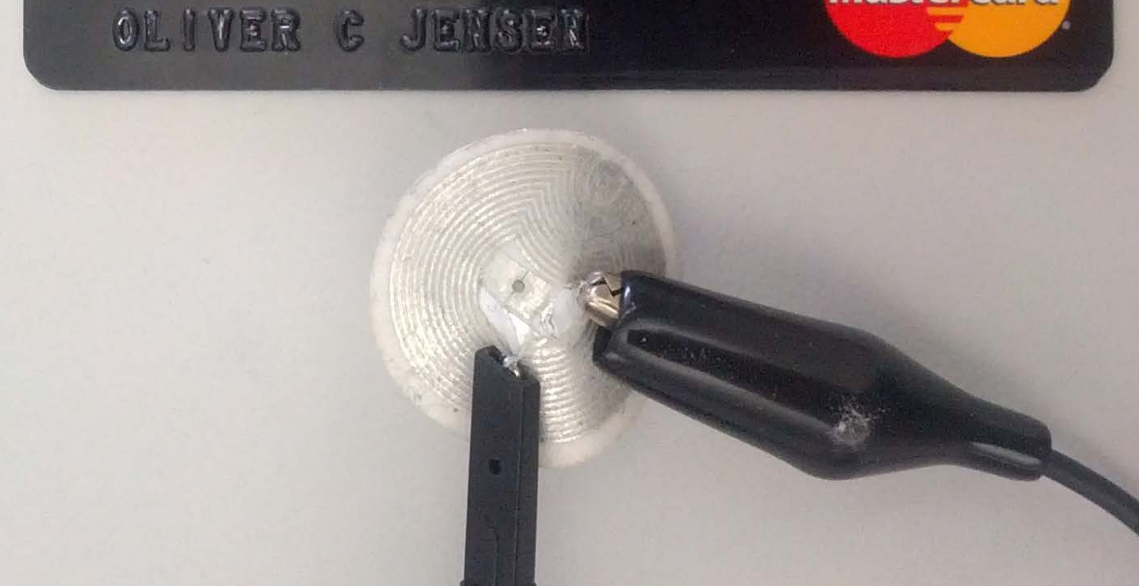
\includegraphics[width=.7\linewidth,height=\textheight,keepaspectratio]{../TomPaper/figures/eavesdroppingAntenna.png}
              \end{center}
              \begin{itemize}
                \pause
                \item{A small antenna could easily be concealed near a terminal}
              \end{itemize}
     \end{minipage}
\end{frame}

\begin{frame}
\frametitle{Skimming \& Relay Attacks}\centering
  \begin{center}
    \includegraphics<1>[width=.7\linewidth,height=\textheight,keepaspectratio]{../TomPaper/figures/CCskim.png}
    \includegraphics<2->[width=.7\linewidth,height=\textheight,keepaspectratio]{../TomPaper/figures/CCskimMask.png}
  \end{center}
    \begin{minipage}{.8\textwidth}
     \vspace{-4mm}
      \begin{block}{The attacker masquerades as a card reader}
        \begin{itemize}
          \item<3->{An unused iCVV can be \textit{skimmed} from the card}
          \item<4->{Then, a fraudulent purchase can occur at a real point of sale}
          \item<5->{In a relay attack, two devices execute the skimming attack in concert}
        \end{itemize}
      \end{block}
    \end{minipage}
\end{frame}


\subsection{Proposed Secure Credit Card Protocol}
\begin{frame}
\frametitle{Proposed Secure Credit Protocol}
 \begin{center}
   \vspace{-8mm}
   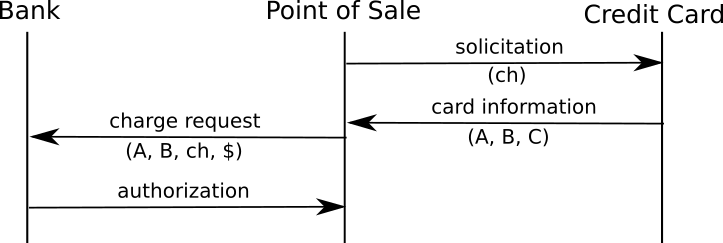
\includegraphics[width=\linewidth,height=.3\textheight,keepaspectratio]{../TomPaper/figures/CCnew.png}
 \end{center}
 \vspace{-6mm}
    \begin{minipage}[t][25mm][t]{\textwidth}
      \only<1>{
        \begin{center}
          \vspace{6mm}
          \begin{minipage}{.6\textwidth}
            \begin{block}{A credit card protocol restructured}\end{block}
          \end{minipage}
        \end{center}
      }
      \only<2>{
        \begin{block}{Solicitation}
          \begin{itemize}
            \item{Point of Sale now sends a challenge}
          \end{itemize}
        \end{block}
      }
      \only<3>{
        \begin{block}{Restructured Card Information}\vspace{2mm}
          \circled{A}~~\textbf{\textit{UUID}}, a static Universally Unique Identifier is used to identify the credit card.\vspace{2mm}\newline
          \circled{B}~~\textit{\textbf{H(card info, ch, iCVV})} is a hash-like function used to authenticate the card's identity.\vspace{2mm}\newline
          \circled{C}~~\textbf{\textit{bank name}} is used to route the charge request.\newline
        \end{block}
      }
      \only<4>{
        \begin{block}{Charge request}
          \begin{itemize}
            \item{Card information is sent to the indicated bank}
          \end{itemize}
        \end{block}
      }
      \only<5>{
        \begin{block}{Authorization}
          \begin{itemize}
            \item{Bank verifies transaction}
          \end{itemize}
        \end{block}
      }
    \end{minipage}
\end{frame}

\begin{frame}
\frametitle{Hash-like function H}\centering
  \begin{minipage}[t][.4\textheight][t]{.8\textwidth}
    \vspace{6mm}
  \begin{block}{Requirements of H}
    \begin{enumerate}
      \item{\textbf{Output appears random} \newline
      Prevents eavesdroppers from gleaning useful information}
      \item{\textbf{Output cannot be used to derive components}\newline
      Protects data. Also, without components, skimmers cannot create a new output that incorporates a new challenge}
    \end{enumerate}
  \end{block}
  \end{minipage}

  \begin{overlayarea}{.6\textheight}{.8\textwidth}
    \begin{center}
      \includegraphics<2>[width=\linewidth,height=\textheight,keepaspectratio]{figures/h50.png}
      \includegraphics<3>[width=\linewidth,height=\textheight,keepaspectratio]{figures/h100.png}
    \end{center}
  \end{overlayarea}
\end{frame}



%-------------------------------------------------------------------
%                           Section
\section{NFC and Mass Transit Ticketing}
\begin{frame}
\frametitle{NFC and Mass Transit Ticketing}
\begin{center}\begin{minipage}{.9\textwidth}
\tableofcontents[currentsubsection, hideothersubsections, sectionstyle=show/shaded]
\end{minipage}\end{center}
\end{frame}
%
%-------------------------------------------------------------------

\begin{frame}
\frametitle{NFC and Mass Transit Ticketing}
  \begin{center}
  \begin{minipage}{.9\textwidth}
  \begin{block}{NFC and Mass Transit Ticketing}
    \begin{itemize}
      \item{Presently, contactless cards widely used for mass transit ticketing}
      \pause
      \vspace{1mm}
      \item{Three Nokia reseachers investigate NFC phone based ticketing}
      \pause
      \vspace{1mm}
      \item{Tamrakar, Ekberg, and Asokan's [2] work is the focus of this section}
      \pause
      \vspace{1mm}
      \item{Their goal is to build a secure ticketing scheme while keeping transaction time below the 300ms industry standard}
    \end{itemize}
  \end{block}
  \end{minipage}
  \end{center}
\end{frame}

% \subsection{Ticketing Architecture}
% \begin{frame}
% \frametitle{Proposed Ticketing Architecture}
% \begin{center}
%   %\begin{minipage}{.9\textwidth}
%   \includegraphics<1>[width=.8\linewidth,height=.8\textheight,keepaspectratio]{figures/ticketing/ticketing55.png}
%   \includegraphics<2>[width=.8\linewidth,height=.8\textheight,keepaspectratio]{figures/ticketing/ticketing60.png}
%   \includegraphics<3>[width=.8\linewidth,height=.8\textheight,keepaspectratio]{figures/ticketing/ticketing65.png}
%   \includegraphics<4>[width=.8\linewidth,height=.8\textheight,keepaspectratio]{figures/ticketing/ticketing70.png}
%   \includegraphics<5>[width=.8\linewidth,height=.8\textheight,keepaspectratio]{figures/ticketing/ticketing75.png}
%   \includegraphics<6>[width=.8\linewidth,height=.8\textheight,keepaspectratio]{figures/ticketing/ticketing80.png}
%   \includegraphics<7>[width=.8\linewidth,height=.8\textheight,keepaspectratio]{figures/ticketing/ticketing85.png}
%   \includegraphics<8>[width=.8\linewidth,height=.8\textheight,keepaspectratio]{figures/ticketing/ticketing90.png}
%   \includegraphics<9>[width=.8\linewidth,height=.8\textheight,keepaspectratio]{figures/ticketing/ticketing95.png}
%   \includegraphics<10>[width=.8\linewidth,height=.8\textheight,keepaspectratio]{figures/ticketing/ticketing100.png}
% %\end{minipage}
% \end{center}
% \end{frame}

\subsection{Ticketing Protocols}
\begin{frame}
\frametitle{Proposed Ticketing Protocol}
\begin{center}
  \includegraphics<1>[width=.8\linewidth,height=.8\textheight,keepaspectratio]{figures/ticketing/protocol0.png}
  \includegraphics<2>[width=.8\linewidth,height=.8\textheight,keepaspectratio]{figures/ticketing/protocol5.png}
  \includegraphics<3>[width=.8\linewidth,height=.8\textheight,keepaspectratio]{figures/ticketing/protocol10.png}
  \includegraphics<4>[width=.8\linewidth,height=.8\textheight,keepaspectratio]{figures/ticketing/protocol15.png}
  \includegraphics<5>[width=.8\linewidth,height=.8\textheight,keepaspectratio]{figures/ticketing/protocol20.png}
  \includegraphics<6>[width=.8\linewidth,height=.8\textheight,keepaspectratio]{figures/ticketing/protocol25.png}
  \includegraphics<7>[width=.8\linewidth,height=.8\textheight,keepaspectratio]{figures/ticketing/protocol30.png}
  \includegraphics<8>[width=.8\linewidth,height=.8\textheight,keepaspectratio]{figures/ticketing/protocol35.png}
  \includegraphics<9>[width=.8\linewidth,height=.8\textheight,keepaspectratio]{figures/ticketing/protocol40.png}
\end{center}
\end{frame}


\begin{frame}
\frametitle{Protocol Variant 1}
  \begin{center}
    \begin{block}{Use a lighter authentication method}
      \begin{itemize}
        % \pause
        % \item{Large RSA keys in certificate are the major cause on long data transfer times}
        \pause
        \item{Switching from a signature to a MAC (\textit{message authentication code}) substantially reduces overhead}
        \pause
      \end{itemize}
    \end{block}
    \begin{block}{Use tokens instead of certificates}
      \begin{itemize}
        \pause
        \item{Send a small token that the reader can validate}
        \pause
        \item{For security, the token should be refreshed often}
      \end{itemize}
    \end{block}
  \end{center}
\end{frame}

\begin{frame}
\frametitle{Protocol Variant 1}
\begin{center}
  \includegraphics<1>[width=.8\linewidth,height=.8\textheight,keepaspectratio]{figures/ticketing/protocol45.png}
  \includegraphics<2>[width=.8\linewidth,height=.8\textheight,keepaspectratio]{figures/ticketing/protocol50.png}
  \includegraphics<3>[width=.8\linewidth,height=.8\textheight,keepaspectratio]{figures/ticketing/protocol55.png}
\end{center}
\end{frame}

\begin{frame}
\frametitle{Protocol Variant 2}
  \begin{center}
    \begin{block}{Use a reversed hash chain}
      \begin{itemize}
        \pause
        \item{Offers timely tokens to be used with a long term certificate}
      \end{itemize}
    \end{block}
  \end{center}
\end{frame}

\subsection{Viability of Mobile Ticketing}

\begin{frame}
\frametitle{Viability of Mobile Ticketing}
  \begin{center}
  \begin{minipage}{.9\textwidth}
    \vspace{-1cm}
    \begin{block}{Viability of Proposed Protocols}
      \begin{table}
        \centering
        %\caption{Estimated protocol speeds}
        \only<1-3>{
          \begin{tabular}{c|c|c|c}
            %RSA
            Encryption Key Size & Standard & Variant 1 & Variant 2\\
            \hline
            1024 bits & 296 ms & 164 ms & 182 ms\\
            1152 bits & 314 ms & 172 ms & 190 ms\\
            2048 bits & 482 ms & 228 ms & 246 ms\\
          \end{tabular}
        }
        \only<4-5>{
          \begin{tabular}{c|c|c|c}
            %RSA
            Encryption Key Size & Standard & Variant 1 & Variant 2\\
            \hline
            \textcolor{uigrey}{1024 bits} & \textcolor{uigrey}{296 ms} & \textcolor{uigrey}{164 ms} & \textcolor{uigrey}{182 ms}\\
            \textcolor{uigrey}{1152 bits} & \textcolor{uigrey}{314 ms} & \textcolor{uigrey}{172 ms} & \textcolor{uigrey}{190 ms}\\
            2048 bits & 482 ms & 228 ms & 246 ms\\
          \end{tabular}
        }
        \only<6>{
          \begin{tabular}{c|c|c|c}
            %RSA
            Encryption Key Size & Standard & Variant 1 & Variant 2\\
            \hline
            \textcolor{uigrey}{1024 bits} & \textcolor{uigrey}{296 ms} & \textcolor{uigrey}{164 ms} & \textcolor{uigrey}{182 ms}\\
            \textcolor{uigrey}{1152 bits} & \textcolor{uigrey}{314 ms} & \textcolor{uigrey}{172 ms} & \textcolor{uigrey}{190 ms}\\
            2048 bits & \textcolor{red}{482 ms} & \textcolor{green}{228 ms} & \textcolor{green}{246 ms}\\
          \end{tabular}
        }
      \end{table}
      \begin{itemize}
        \item<2->{NFC transfer speeds were the biggest bottleneck}
        \item<3->{The authors noted that smaller two key sizes have been deprecated in the payment industry}
        \item<5->{After taking the 300ms goal into account, only two options are viable}
      \end{itemize}
    \end{block}
  \end{minipage}
  \end{center}
\end{frame}

\begin{frame}
\frametitle{Viability of Mobile Ticketing}
  \begin{center}
  \begin{minipage}{.9\textwidth}
    \begin{block}{Viability of Mobile Ticketing}
        \begin{itemize}
        \item{Using mobile ticketing offers convince and a richer user interface}
        \pause
        \vspace{1mm}
        \item{The Nokia researchers grant that relay attacks are possible in all protocols, but that there is a short opportunity windows and low monetary gain }
                %  \begin{enumerate}
                %    \item{Tokens and hash-chain values limit window of opportunity}
                %    \item{Public nature of transit stations make such attacks less attractive}
                %    \item{Inexpensive tickets aren't likely worth stealing}
                %  \end{enumerate}
        \pause
        \vspace{1mm}
        \item{The authors state that these protocols are meets performance and security needs better than the current contactless card system}
        \pause
        \vspace{1mm}
        \item{While mobile ticketing is an imperfect, it is valid path forward that offers value}
      \end{itemize}
    \end{block}
  \end{minipage}
  \end{center}
\end{frame}


%-------------------------------------------------------------------
%                           Section
\section{EnGarde: Physical NFC Security}
\begin{frame}
\frametitle{EnGarde: Physical NFC Security}
\begin{center}\begin{minipage}{.9\textwidth}
\tableofcontents[currentsubsection, hideothersubsections, sectionstyle=show/shaded]
\end{minipage}\end{center}
\end{frame}
%
%-------------------------------------------------------------------

\begin{frame}
\frametitle{EnGarde: Physical NFC Security}
  \begin{center}
  \begin{minipage}{.9\textwidth}
  \begin{block}{EnGarde: Physical NFC Security}
    \begin{itemize}
      \item{Commercial payments systems are bringing NFC to phones}
      \pause
      \vspace{1mm}
      \item{As a result, there may be new risks in both payment and non-payment applications of NFC}
      \pause
      \vspace{1mm}
      \item{EnGarde is a semi-permanent phone attachment, designed to act as a hardware-based firewall}
      \pause
      \vspace{1mm}
      \item{EnGarde's logic is independent from phone OS, and can be updated to combat current and future threats}
      \pause
      \vspace{1mm}
      \item{Gummeson et al's [3] work on the EnGarde prototype is the focus of this section}
    \end{itemize}
  \end{block}
  \end{minipage}
  \end{center}
\end{frame}


\begin{frame}
\frametitle{EnGarde Expectations}
  \begin{center}

    \begin{block}{EnGarde should defend against all NFC modes}
      \begin{center}

        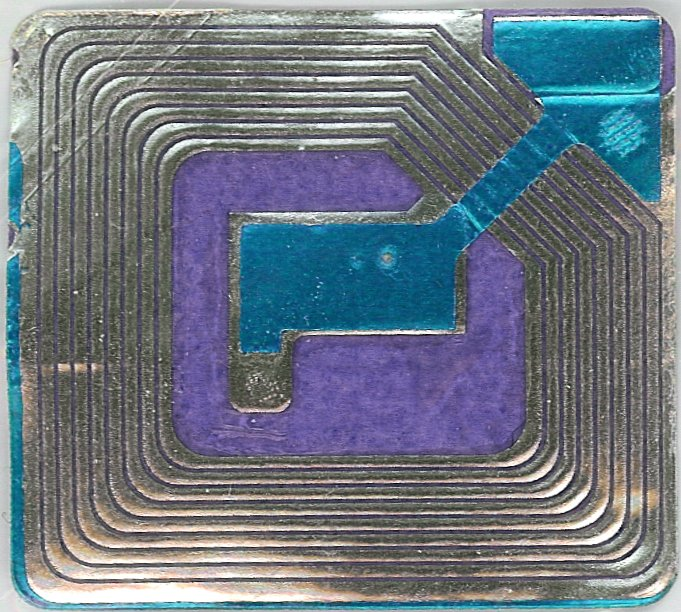
\includegraphics[width=\linewidth,height=0.3\textheight,keepaspectratio]{figures/wikimediatag.jpg}
        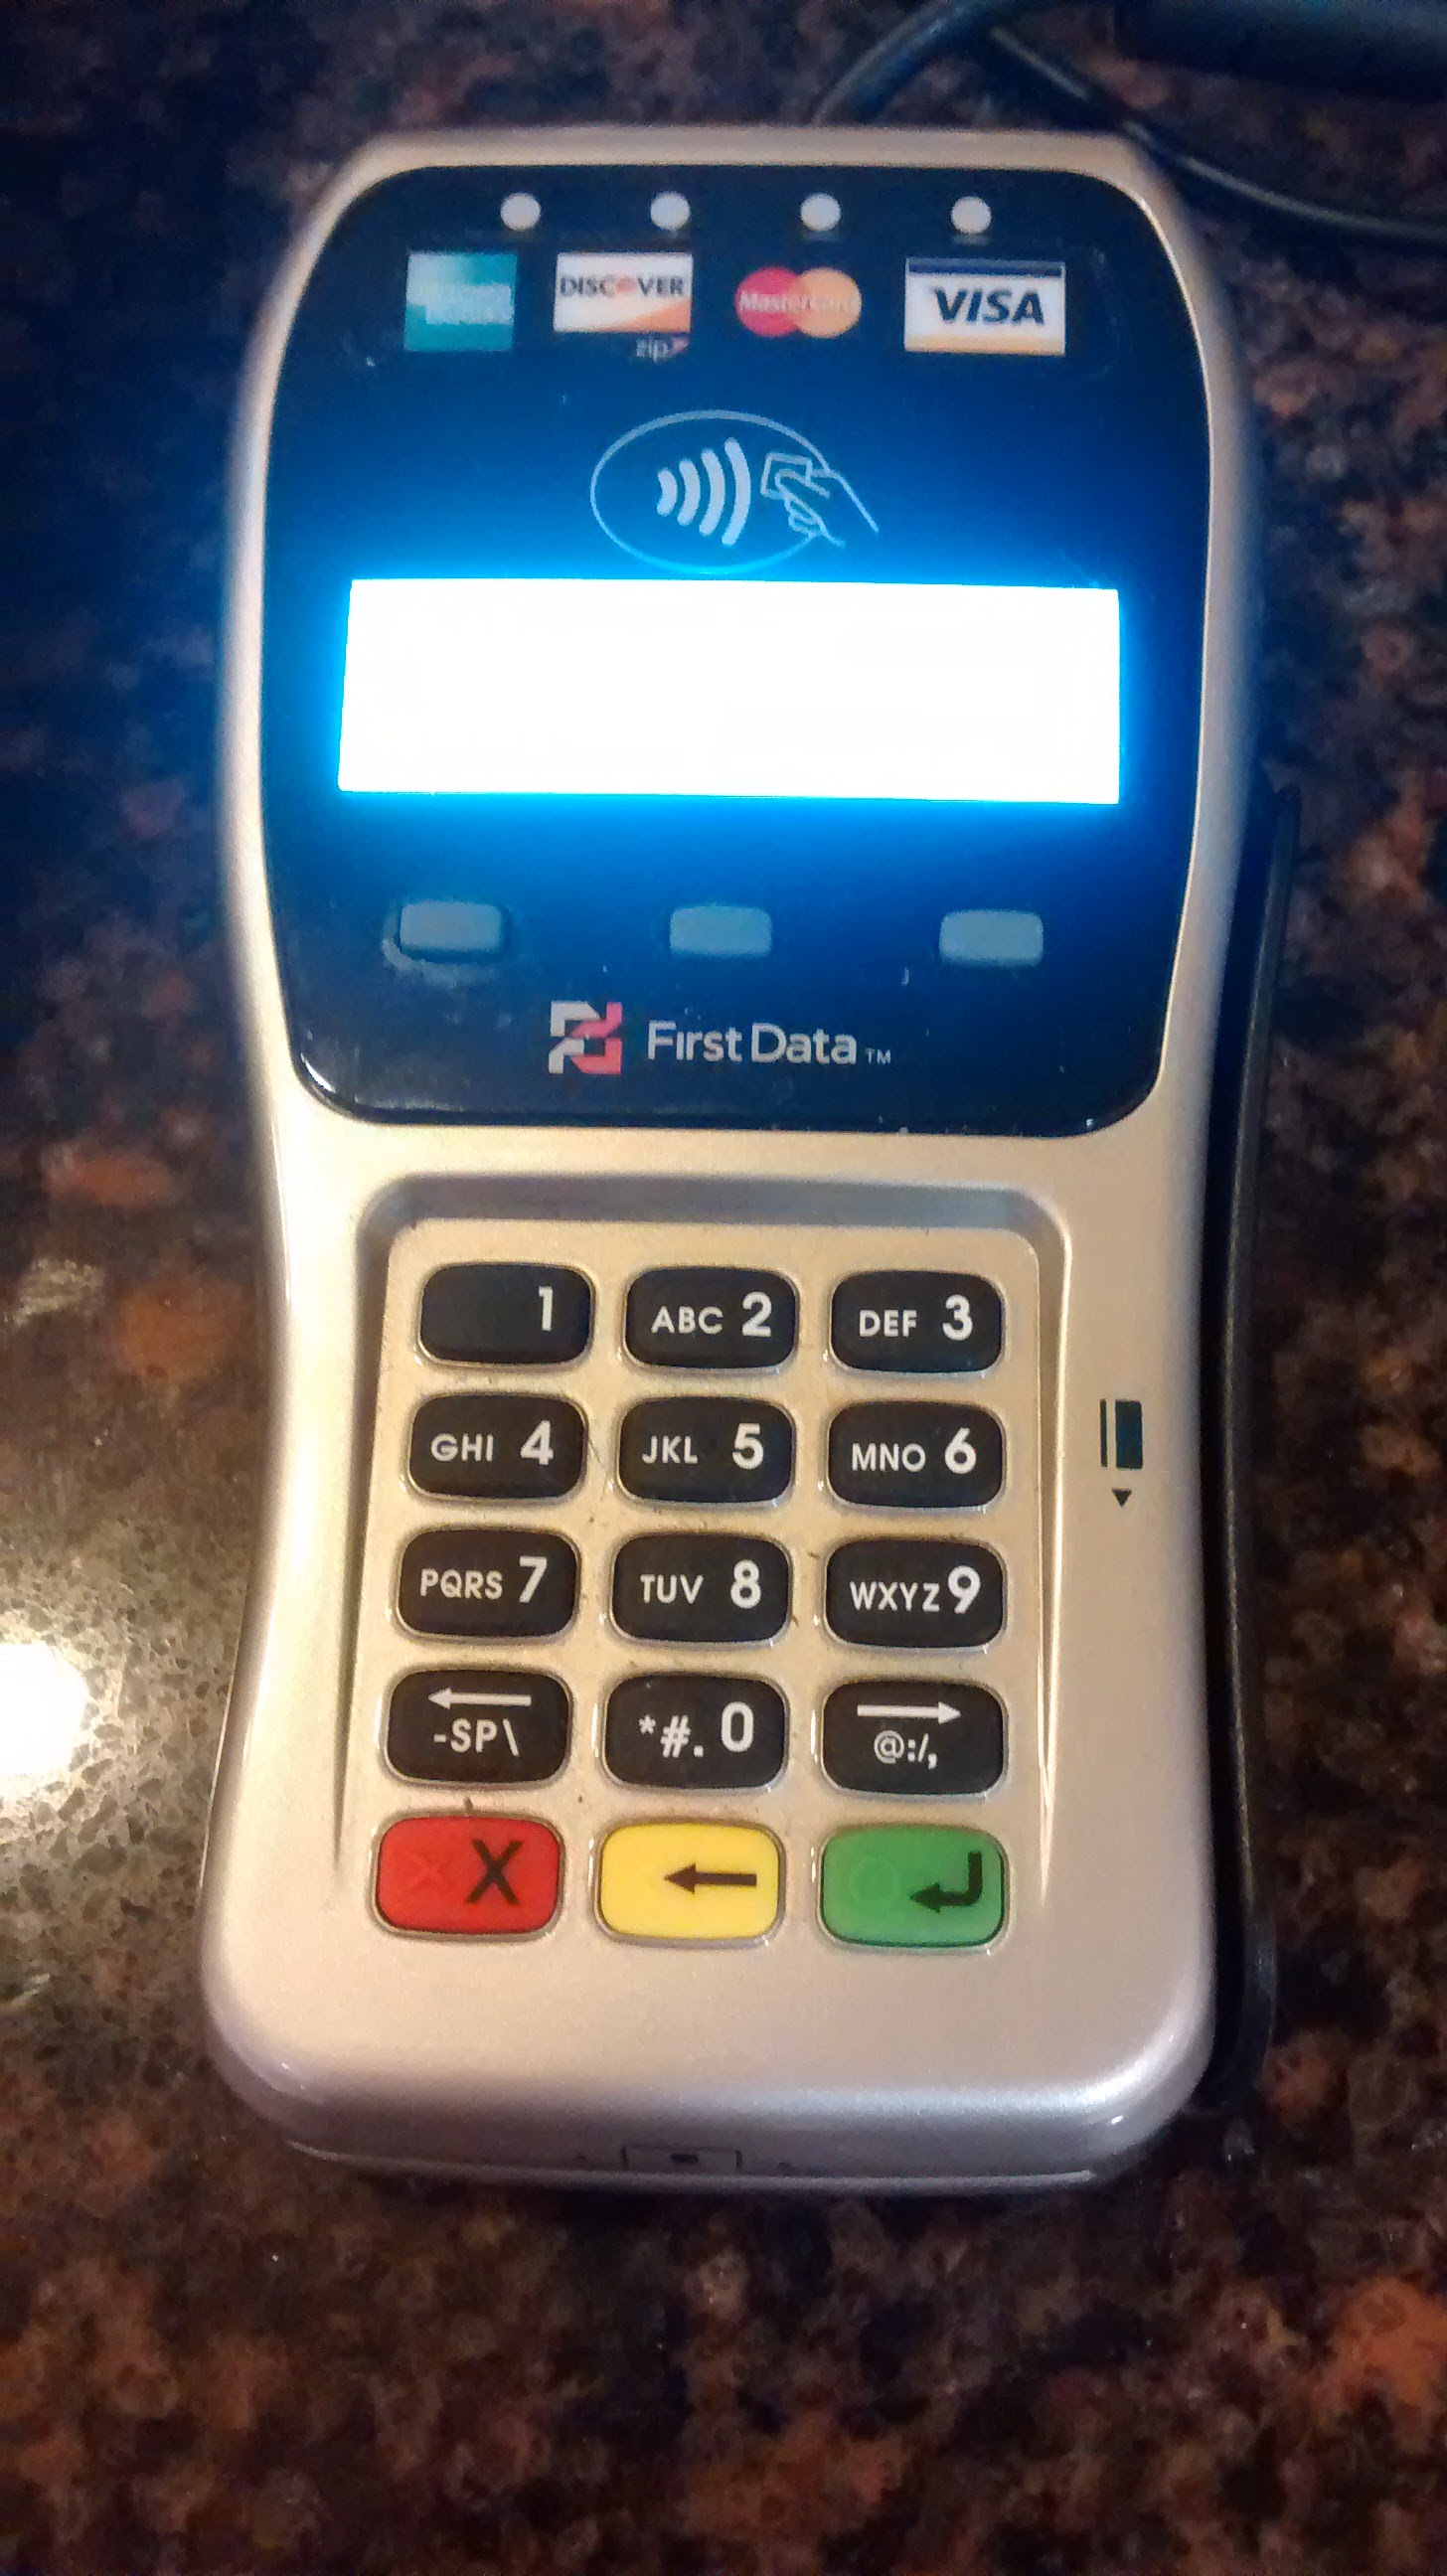
\includegraphics[width=\linewidth,height=0.3\textheight,keepaspectratio]{figures/higbies.jpg}
        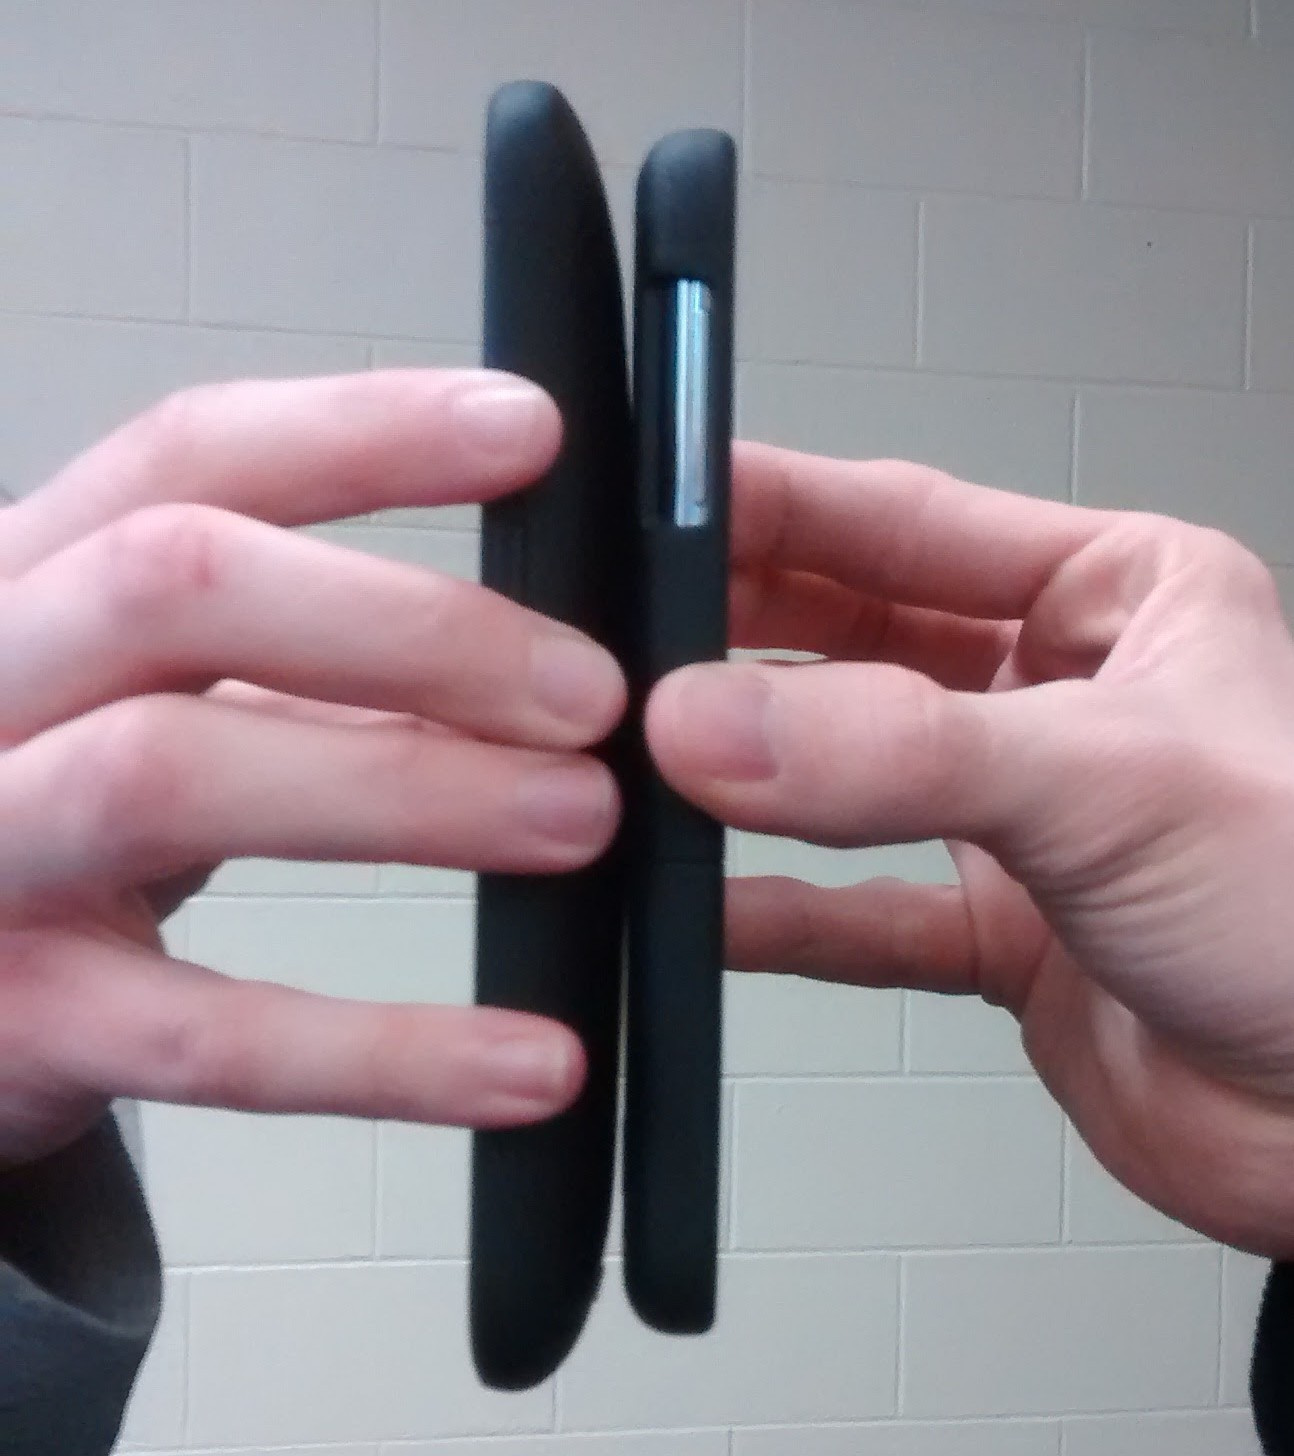
\includegraphics[width=\linewidth,height=0.3\textheight,keepaspectratio]{figures/peer.jpg}

        \vspace{3mm}

        \begin{minipage}{.7\textwidth}
          \begin{itemize}
            \item{Malicious tags}
            \item{Malicious readers}
            \item{Malicious peers}
            \item{Malicious software installations}
          \end{itemize}
        \end{minipage}

      \end{center}
    \end{block}
  \end{center}
\end{frame}



% \begin{center}\textcolor{uipoppy}{We will describe each mode as we go}\end{center}\vspace{3mm}
\begin{frame}
\frametitle{EnGarde State Diagram}
\begin{center}
  \includegraphics<1>[width=.8\linewidth,height=.7\textheight,keepaspectratio]{figures/engarde/states1.png}
  \includegraphics<2>[width=.8\linewidth,height=.7\textheight,keepaspectratio]{figures/engarde/states1a.png}%%we'll start with No Power (flip)
\end{center}
\end{frame}


\subsection{No Power}
\begin{frame}
\frametitle{EnGarde State: No Power}
  \begin{center}
  \begin{minipage}{.9\textwidth}
  \begin{block}{No Power}
    \begin{itemize}
      \item{EnGarde has its own battery independent from the phone, therefore it can encounter a No Power state}
      \pause
      \vspace{1mm}
      \item{To maintain a charge, EnGarde harvests power from NFC communication}
      \pause
      \vspace{1mm}
      \item{Even if EnGarde is completely dead, it will fail safely}
      \pause
    \end{itemize}
  \end{block}
  \end{minipage}
  \end{center}
\end{frame}



\begin{frame}
\frametitle{EnGarde State Diagram}
\begin{center}
  \includegraphics<1>[width=.8\linewidth,height=.7\textheight,keepaspectratio]{figures/engarde/states2.png}
  \includegraphics<2>[width=.8\linewidth,height=.7\textheight,keepaspectratio]{figures/engarde/states2a.png}%%we'll start with No Power (flip)
\end{center}
\end{frame}


\subsection{System Idle}
\begin{frame}
\frametitle{EnGarde State: System Idle}
  \begin{center}
  \begin{minipage}{.9\textwidth}
  \begin{block}{System Idle}
    \begin{itemize}
      \item{EnGarde maintains charge}
      \pause
      \vspace{1mm}
      \item{EnGarde waits}
    \end{itemize}
  \end{block}
  \end{minipage}
  \end{center}
\end{frame}

\begin{frame}
\frametitle{EnGarde State Diagram}
\begin{center}
  \includegraphics<1>[width=.8\linewidth,height=.7\textheight,keepaspectratio]{figures/engarde/states3.png}
  \includegraphics<2>[width=.8\linewidth,height=.7\textheight,keepaspectratio]{figures/engarde/states3a.png}%%we'll start with No Power (flip)
\end{center}
\end{frame}



\subsection{NFC Decoder Active}
\begin{frame}
\frametitle{EnGarde State: Decoder Active}
  \begin{center}
  \begin{minipage}{.9\textwidth}
  \begin{block}{NFC Decoder Active}
    \begin{itemize}
      \item{There is an incoming or outgoing transmission. EnGarde must listen...}
      \pause
      \vspace{1mm}
      \item{EnGarde scans transmissions and determines if they are worthy using a set of blocking rules}
      \pause
      \vspace{1mm}
      \item{The blocking rules can be updated for robust handling of current and future attacks}
    \end{itemize}
  \end{block}
  \end{minipage}
  \end{center}
\end{frame}



\begin{frame}
\frametitle{EnGarde State Diagram}
\begin{center}
  \includegraphics<1>[width=.8\linewidth,height=.7\textheight,keepaspectratio]{figures/engarde/states4.png}
  \includegraphics<2>[width=.8\linewidth,height=.7\textheight,keepaspectratio]{figures/engarde/states4a.png}%%we'll start with No Power (flip)
\end{center}
\end{frame}

\subsection{Jam Mode}
\begin{frame}
\frametitle{EnGarde State: Jammer}
  \begin{center}
  \begin{minipage}{.9\textwidth}
  \begin{block}{Reflective Jamming}
    \begin{itemize}
      \item{This jamming method is used against low-powered tags}
      \pause
      \vspace{1mm}
      \item{By broadcasting on the same frequency, EnGarde can block out messages from malicious tags}
      \pause
      \vspace{1mm}
      \item{The power the phone is using to activate the tags also powers EnGarde's defense}
    \end{itemize}
  \end{block}
  \end{minipage}
  \end{center}
\end{frame}

\begin{frame}
\frametitle{EnGarde State: Jammer}
  \begin{center}
  \begin{minipage}{.9\textwidth}
  \begin{block}{Pulse Jamming}
    \begin{itemize}
      \item{This jamming method is used against high-powered readers or peers}
      \pause
      \vspace{1mm}
      \item{Since a reader is sourcing a considerable amount of power, Engarde can only corrupt rather than completely block messages}
      \pause
      \vspace{1mm}
      \item{The power from the reader sustains EnGarde's defense}
    \end{itemize}
  \end{block}
  \end{minipage}
  \end{center}
\end{frame}


\begin{frame}
\frametitle{EnGarde State Diagram}
\begin{center}
  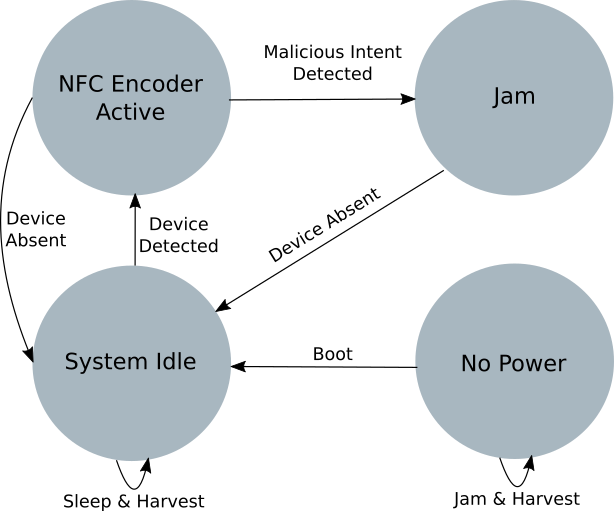
\includegraphics[width=.8\linewidth,height=.7\textheight,keepaspectratio]{figures/engarde/states5.png}
\end{center}
\end{frame}

\subsection{Experimental Evaluation of EnGarde}

\begin{frame}
\frametitle{Experimental Evaluation of EnGarde}
  \begin{center}
  \begin{minipage}{.9\textwidth}
  \begin{block}{Jamming}
    \begin{itemize}
      \item{EnGarde was able to successfully block all malicious test cases using one of the jamming methods}
      \pause
      \vspace{1mm}
      \item{Decoding was also successful in decoding a malicious tag to URL \textit{http://www.malware}}
      \pause
      \vspace{1mm}
      \item{EnGarde's defense seems strong, but we note that its defense is only as strong as the blocking rules it has}
    \end{itemize}
  \end{block}
  \end{minipage}
  \end{center}
\end{frame}

%-------------------------------------------------------------------
%                           Section
\section{Conclusion}
\begin{frame}
\frametitle{Conclusion}
\begin{center}\begin{minipage}{.9\textwidth}
\tableofcontents[currentsubsection, hideothersubsections, sectionstyle=show/shaded]
\end{minipage}\end{center}
\end{frame}
%
%-------------------------------------------------------------------

\begin{frame}
\frametitle{Conclusion}
  \begin{center}
  \begin{minipage}{.9\textwidth}
  \begin{block}{Conclusion}
    \begin{itemize}
      \item{If we are clever, we can have secure contactless credit cards}
      \pause
      \vspace{1mm}
      \item{NCF ticketing is a viable option for the future, but NFC data transfer speeds need improvement}
      \pause
      \vspace{1mm}
      \item{EnGarde's defense seems strong, but we note that its defense is only as strong as the blocking rules it has}
    \end{itemize}
  \end{block}
  \end{minipage}
  \end{center}
\end{frame}

\begin{frame}
  \frametitle{Questions}
  \begin{center}
    {\huge \textcolor{uipoppy}{Questions?}}\\*
    %\includegraphics[width=.2\linewidth,height=.2\textheight,keepaspectratio]{figures/tinfoil.png}\\*
    %\textcolor{uipaleblue}{Tinfoil Hats for Everyone!}\\*
      % \begin{minipage}{.6\textwidth}
        \vspace{.7cm}
        \textcolor{uipaleblue}{\textit{Stop by the NFC enabled pop machine near the bookstore for a neat demonstration.}}
      % \end{minipage}
\end{center}
\end{frame}

\begin{frame}
  \frametitle{Sources}
  \begin{block}{Primary Research Sources}
    \begin{enumerate}
      \item{Oliver Jensen, Mohamed Gouda, and Lili Qiu. 2016. A secure credit card protocol over NFC. In Proceedings of the 17th International Conference on Distributed Computing and Networking (ICDCN '16). ACM, New York, NY, USA, Article 32 , 9 pages. %DOI=http://dx.doi.org.ezproxy.morris.umn.edu/10.1145/2833312.2833319
      }
      \item{Sandeep Tamrakar, Jan-Erik Ekberg, and N. Asokan. 2011. Identity verification schemes for public transport ticketing with NFC phones. In Proceedings of the sixth ACM workshop on Scalable trusted computing (STC '11). ACM, New York, NY, USA, 37-48. %DOI=http://dx.doi.org.ezproxy.morris.umn.edu/10.1145/2046582.2046591
      }
      \item{Jeremy J. Gummeson, Bodhi Priyantha, Deepak Ganesan, Derek Thrasher, and Pengyu Zhang. 2013. EnGarde: protecting the mobile phone from malicious NFC interactions. In Proceeding of the 11th annual international conference on Mobile systems, applications, and services (MobiSys '13). ACM, New York, NY, USA, 445-458. %DOI=http://dx.doi.org.ezproxy.morris.umn.edu/10.1145/2462456.2464455
      }
    \end{enumerate}
  \end{block}
\end{frame}

\begin{frame}
  \frametitle{Sources}
  \begin{block}{Additional Sources}
    \begin{itemize}
      \item{Personal photos
      }
      \item{Wikipedia}
      \item{Robert Hardy, Enrico Rukzio, Paul Holleis, and Matthias Wagner. 2010. Mobile interaction with static and dynamic NFC-based displays. In Proceedings of the 12th international conference on Human computer interaction with mobile devices and services (MobileHCI '10). ACM, New York, NY, USA, 123-132. %DOI=http://dx.doi.org.ezproxy.morris.umn.edu/10.1145/1851600.1851623
      }
    \end{itemize}
  \end{block}
\end{frame}


%-------------------------------------------------------------------
%                          Sample Slide
%-------------------------------------------------------------------

%\begin{frame}
%    \frametitle{Elements in Whoville}
%
%    \vspace{1cm} % generate some space between title and content
%    \begin{table}[h]
%    \centering
%    \begin{tabular}{lcccc} \bottomrule[2pt]
%        Name & Symbol & $A_r$ & M.P. (K) & IE (J) \\ \bottomrule
%        Helium & He & $4.00$ & $1$ & $3.94e^{-18}$ \\
%        Carbon & C & $12.01$ & $773$ & $3.94e^{-18}$ \\
%        Arsenic & As & $74.92$ & $1090$ & $1.48e^{-18}$ \\
%        Gold & Au & $196.96$ & $1337$ & $1.48e^{-18}$ \\
%        Cobalt & Co & $58.93$ & $1495$ & $1.26e^{-18}$ \\
%    \bottomrule[2pt]
%    \end{tabular}
%    \caption{Properties of Whoville Elements}
%    \end{table}
%
%\vspace{-0.6cm} % compact spacing between table and text
%
%    \begin{columns}[t]
%    \column{4.5cm}
%    \begin{block}{Trace rare earth metals:}
%    \begin{itemize}
%        \item{Ytterbium}
%        \item{Praseodymium}
%        \item{Neodymium}
%    \end{itemize}
%    \end{block}
%    \column{4.5cm}
%    \begin{block}{Obtaining Neodymium:}
%        \vspace{0.15cm}
%        \circled{1}$\textemdash$bastn\"{a}site \\
%        \circled{2}$\textemdash${monazite} \\
%    \end{block}
%    \end{columns}
%
%    \textref{Dr. Seuss et al. 2011}
%
%\end{frame}

\end{document}
